
%%%%%%%%%%%%%%%%%%%%% Results %%%%%%%%%%%%%%%%%%%%%%%%%%%%%%%%%%%

\section{Results}

\subsection{Transcriptome data in the Primary blood Cancer Cell encyclopedia (PACE)} 

\subsubsection{Occurence of genetic variants}
PACE includes transcriptome data from 184 CLL patients. In total PACE covers 89 single genetic variants composed of 68 gene mutations and 21 CNVs. Many samples showed multiple variants, which is in line with previous characterization of CLL \citep{Landau2015}. In this study we focused on the most common variants with a prevalence of $> 3.5\%$ resulting in 6 CNVs and 7 gene mutations. Del13q14 was the most common variant with 113 cases. 79 samples were hypermutated in the IGHV gene and 96 had an unmutated IGHV locus. Trisomy12 and TP53 appeared in 23 resp.\ 30 samples.  Figure \ref{fig:tableOverview} shows the occurrence of genetic variants dependent on the sample's IGHV status indicating correlations and anti-correlations between variants. $\chi^2$-squared tests revealed significantly high or low co-occurrence of 8 variant pairs. We found TP53 and Del17p13 highly correlated, as well as Del8p12 and Gain8q24, which are both located on chromosome 8. Hypermutated IGHV was associated with Del11q22.3 and TP53, while Trisomy12 was exclusive for Del13q14 (Figure~\ref{fig:corplot_Chisquare}). 

%\begin{figure}
%	\centering
%	\def\svgwidth{\columnwidth}
%	\input{./Figures/data_overview.pdf_tex}
%	\caption{\textbf{Overview Genetic variants in PACE:} Distribution of the most common genetic variants in the 184 CLL patients included in the PACE transcriptome data set. 6 genetic abberations and 7 gene mutations were have a prevalence of $> 3.5\%$.}
%	\label{fig:Overview}
%\end{figure}       


\begin{figure}
	\centering
	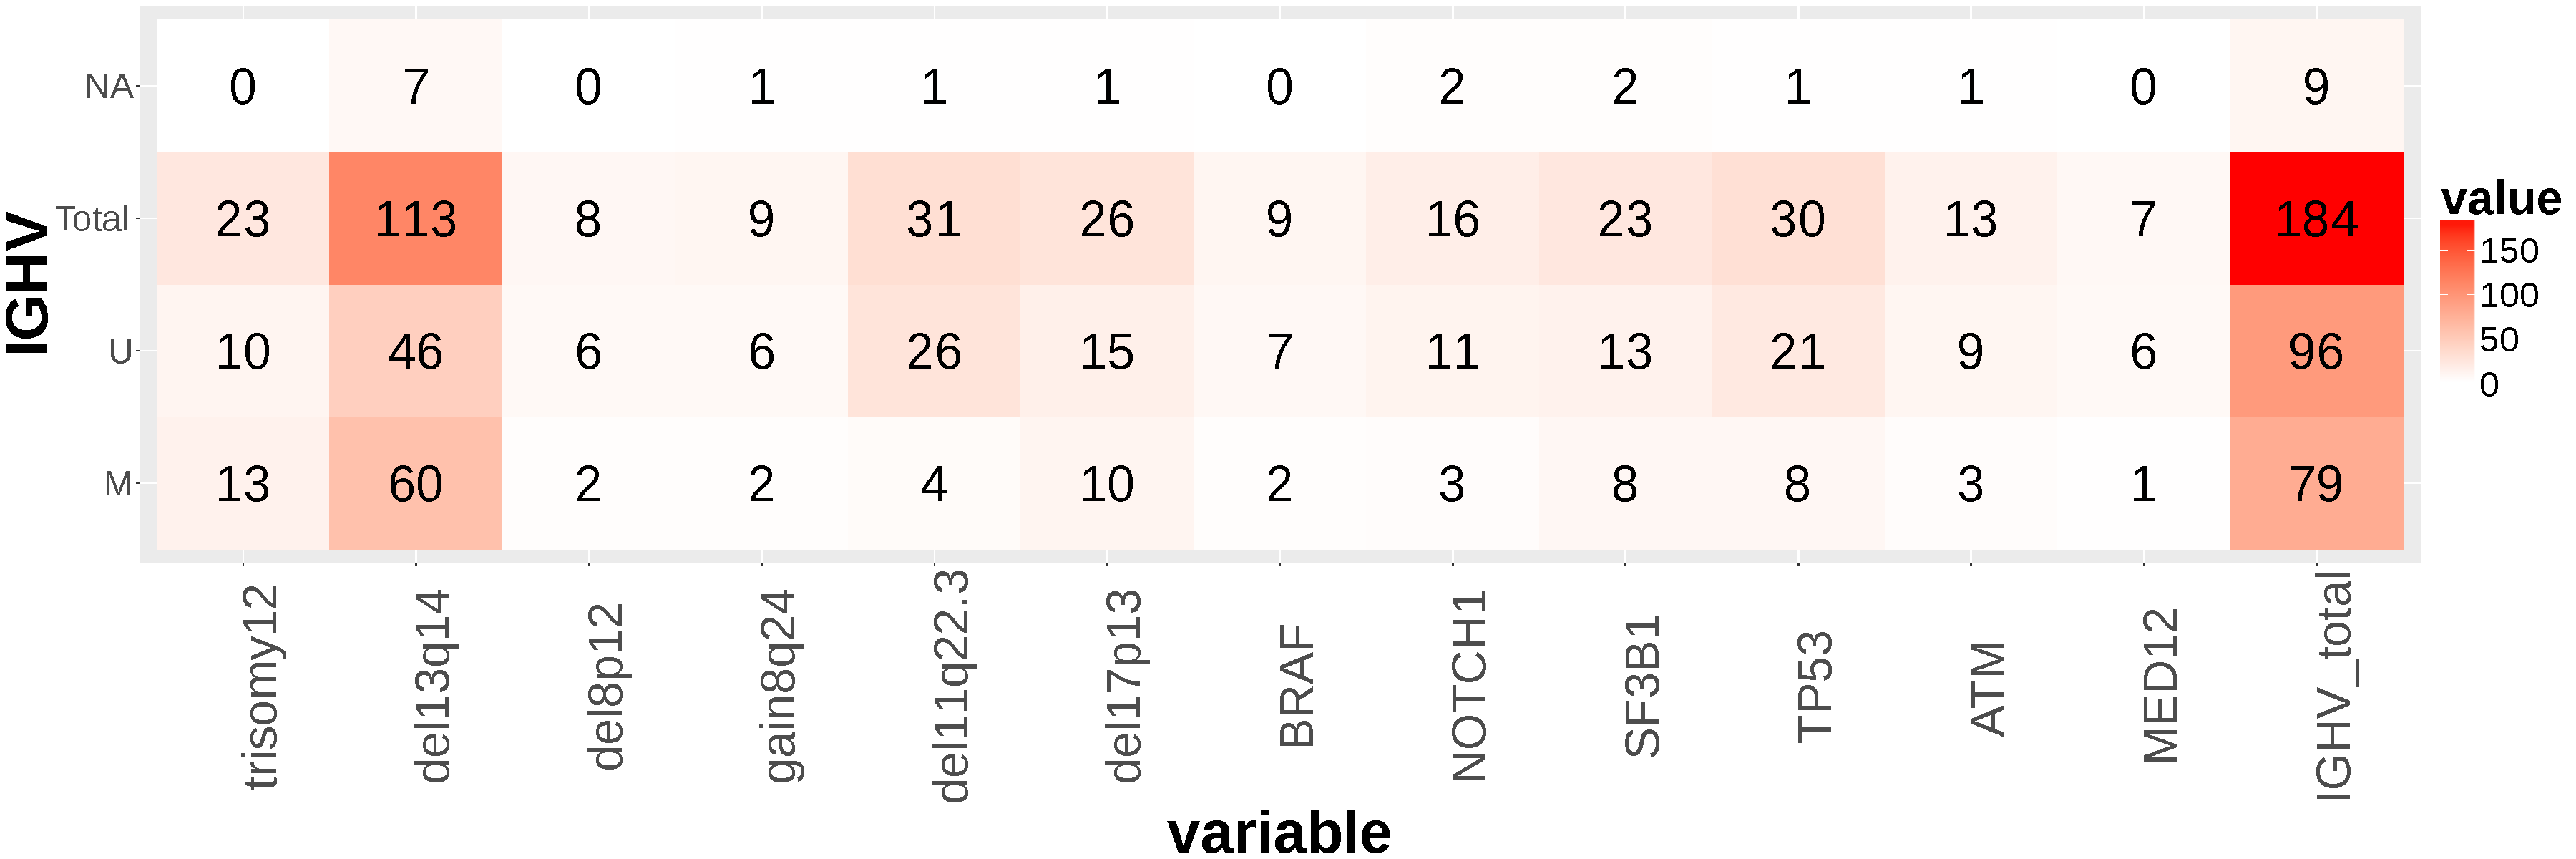
\includegraphics[width=\columnwidth]{./Figures/datatable_overview.pdf}
	\caption{\textbf{Variants in PACE samples by IGHV status:} Most common genetic variants in CLL samples from the PACE transcriptome data set. The distribution by IGHV status for each variant differs, revealing biases and interactivity between variants.}
	\label{fig:tableOverview}
\end{figure}
         

\begin{figure}
	\centering
	\def\svgwidth{\columnwidth}
	\input{./Figures/corplot_chiquare.pdf_tex}
	\caption{\textbf{Co-occurrence of genetic variants:} -log10(pvalue) for co-occurrence of genetic variants calculated by $\chi^2$-square test. The sign indicates the direction of association. Del17p13 and TP53, Del8p12 and Gain8q24, as well as Del11q22.3 and IGHV and Trisomy12 and Del13q14 are significantly associated or excluding.}
	\label{fig:corplot_Chisquare}
\end{figure} 

\FloatBarrier

\subsubsection{IGHV status and Trisomy12 form distinct gene expression cluster}
Genetic profiling of CLL unraveled a variety of driver mutations and genomic features in relation to the disease's phenotypes. Here we aimed to study characteristics of these genetic profiles on transcriptome level. First, we determined the influence of genetic variation on gene expression and thus the capability of PACE to identify specific expression signatures. Hierarchical clustering by the 5000 most variant genes separated samples first by their IGHV status. Samples were further subdivided into the three methylation cluster, which had been classified on the basis of methylome data. Within IGHV groups the Trisomy12 formed sub cluster also revealed a distinct expression pattern. Other variants as TP53, Del11q22.3 and Del13q14 were less connected, but formed several sub cluster with some independent samples. Altogether, clustering revealed an overlap on transcriptome level within different samples based on gene variants (Figure \ref{fig:cluster500exprGenes}).

\begin{figure}
	\centering
	\def\svgwidth{\columnwidth}
	\input{./Figures/cluster500exprgenes.pdf_tex}
	\caption{\textbf{Hierarchical clustering of CLL samples based on the 5000 most variable genes:} Unsupervised sample clustering based on the 5000 most variable genes reveals distinct cluster separated by IGHV status, Methylation groups and Trisomy12.}
	\label{fig:cluster500exprGenes}
\end{figure}


\FloatBarrier

\subsubsection{RNA preparation method, IGHV status and Trisomy12 explain major parts of gene expression variance}

We performed principal component analysis (PCA) to asses to which extend genetic features contribute to the variance of gene expression data. T-test for associations between genetic variants and principal components revealed IGHV status, Trisomy12 and RNA preparation method as main factors to explain genetic variance (Figure \ref{fig:corplot_pca_variants}). Other variants like TP53, Del13q14 and Del11q22 also showed significant associations with one of the first principal components, but correlation and anti-correlation of variants confounded detailed evaluation (see Occurrence of genetic variants). The first principal component (PC1) was associated with the RNA preparation method (Figure \ref{fig:pca}A). Probes collected from a pellet were separated from those extracted by CD19+ selection. CD19 is a B cell marker and selection by CD19+ cells should reduce contamination with other cell types as T cells \citep{Abbasi-Kenarsari2015}. Contamination with other cell types is a common problem in blood cancer samples and we corrected for this as confounding factor in further analyses (see T-cell contamination). 
In line with hierarchical clustering, the second principal component (PC2) displayed IGHV and methylation status, as both are highly correlated (Figure \ref{fig:pca}B/C). Trisomy12 was associated with PC3 and PC4, which still represented 6.2\% and 4.2 \% of the variance (Figure \ref{fig:pca}D). Later principal components like PC9 and PC10 were significantly associated with MED12 and Del17p13, but accounted for less than 2\% of the variance.
Beside their function for quality control these findings validate the suitability of PACE to analyze transcriptional profiles.  

\begin{figure}
	\centering
	\def\svgwidth{\columnwidth}
	\input{./Figures/corplot_pca_variants.pdf_tex}
	\caption{\textbf{Association of genetic variants and principal components:} -log10 (pvalue) t-test for correlation between genetic variants and principal components. PC1 was found to be associated with RNA preparation method and PC2 with IGHV and Del11q22.3. PC3 and PC4 show both significant correlation with Trisomy12 status.}
	\label{fig:corplot_pca_variants}
\end{figure} 

\begin{figure}
	\centering
	\begin{subfigure}[t]{0.45\columnwidth}
		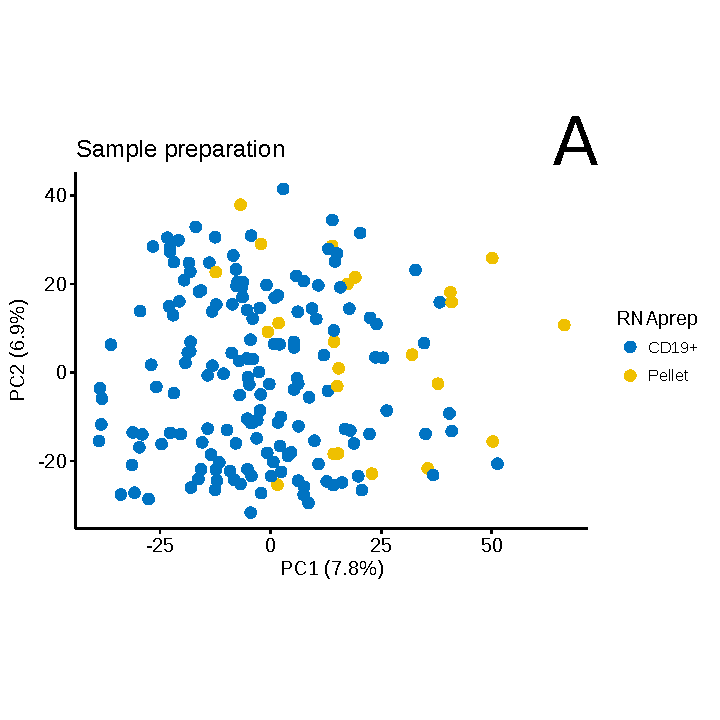
\includegraphics[width=\columnwidth]{./Figures/pca_RNAprep.pdf}
		%\input{./Figures/pca_RNAprep.pdf_tex}
		\subcaption*{}
		\label{fig:pca_RNAprep}
	\end{subfigure}
	\quad
	%add desired spacing between images, e. g. ~,def\svgwidth{\columnwidth} \quad, \qquad, \hfill etc. 
	%(or a blank line to force the subfigure onto a new line)
	\begin{subfigure}[t]{0.45\columnwidth}
		%\def\svgwidth{\columnwidth}
		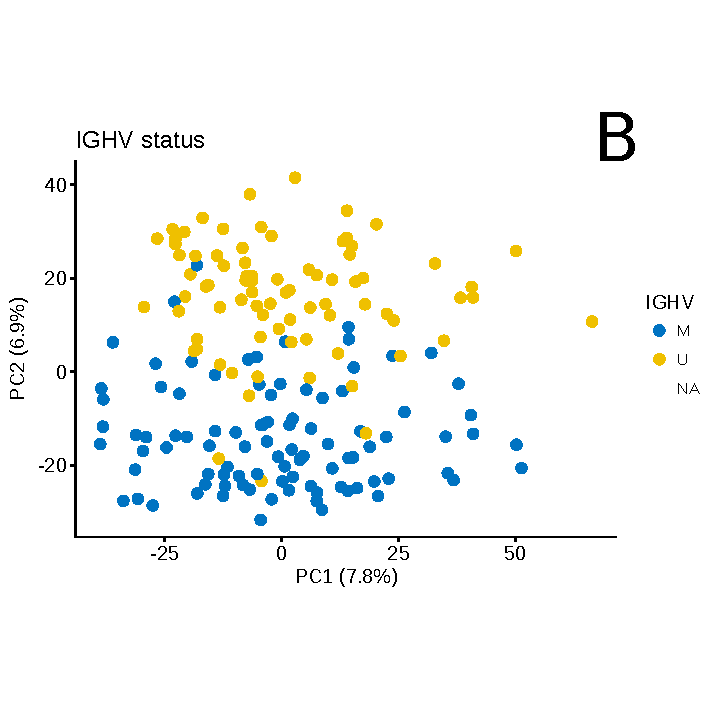
\includegraphics[width=\columnwidth]{./Figures/pca_ighv_test.pdf}
		%\input{./Figures/pca_ighv.pdf_tex}
		\subcaption*{}
		\label{fig:pca_IGHV}
	\end{subfigure}
	\quad
	\begin{subfigure}[t]{0.45\columnwidth}
		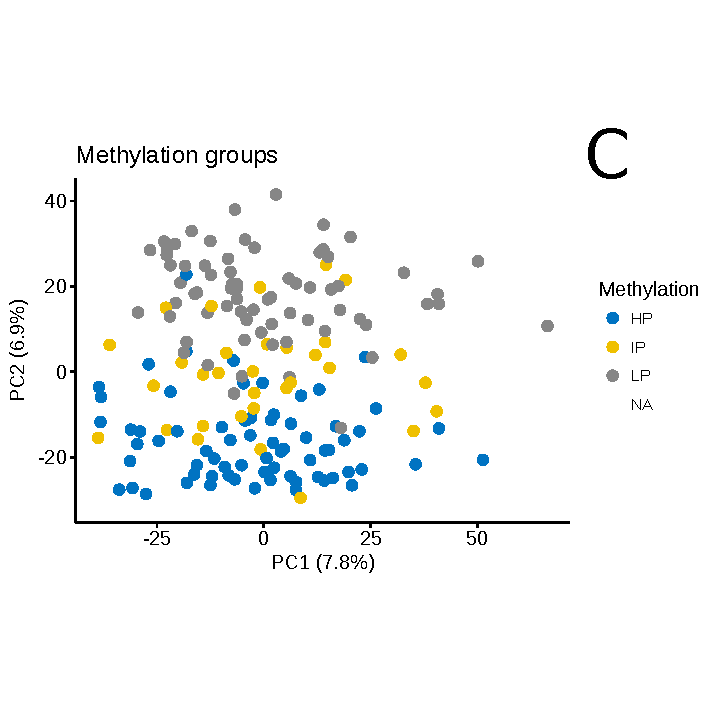
\includegraphics[width=\columnwidth]{./Figures/pca_Methylation.pdf}
		\subcaption*{}
		\label{fig:pca_Methylation}
	\end{subfigure}
	\quad
	\begin{subfigure}[b]{0.45\columnwidth}
		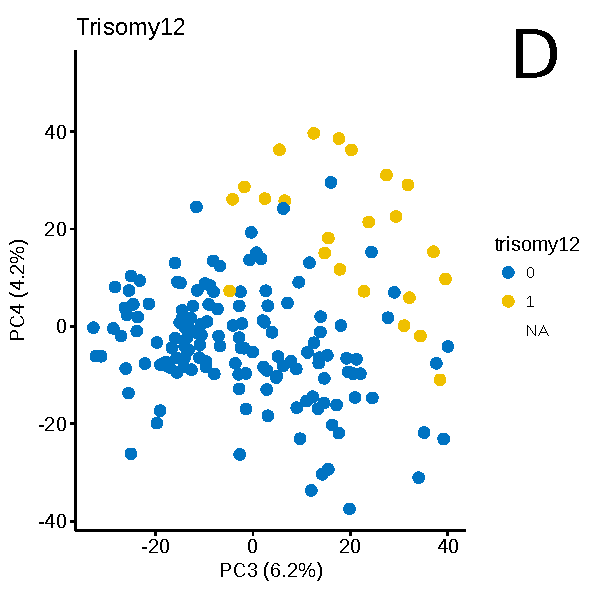
\includegraphics[width=0.8\columnwidth]{./Figures/pca_trisomy12.pdf}
		\subcaption*{}
		\label{fig:pca_trisomy12}
	\end{subfigure}
	\caption{\textbf{Principal component analysis by 5000 most variant genes:} \textbf{(A)} PC1 reflect highest variability within PACE cohort. It correlates with RNA preparation method, which reflects the degree of T-cell contamination. \textbf{(B)} IGHV status is associated with PC2. \textbf{(C)} Methylation groups further refine IGHV distinction. \textbf{(D)} Trisomy12 sample cluster on PC3 and PC4 }
	\label{fig:pca}
\end{figure}


\FloatBarrier

\subsubsection{Confounding factors}

\subsubsection{Batch effects by adapter contamination}
Transcriptome data in PACE were collected over a period of more than four years. During this time sequencing machines and platform were changed enabling to sequence longer reads. These changes in read length were reflected in distinct sample clustering in exploratory data analysis (Figure \ref{fig:Trimming}A). Cluster also correlated with the library adapter contamination. Longer reads showed an increased number of adapters as shown in Figure \ref{fig:adapter_contam}. As insert size distribution of sequenced reads was equal among samples, but read length increased with platform changes, the probability of sequencing into the adapter sequence increased as well. Adapter sequences can infer mapping biases or even lead to mismapping \citep{Sturm}. Thus, adapters were trimmed before mapping, removing the batch effect (Figure \ref{fig:Trimming}B).   

\begin{figure}
	\centering
	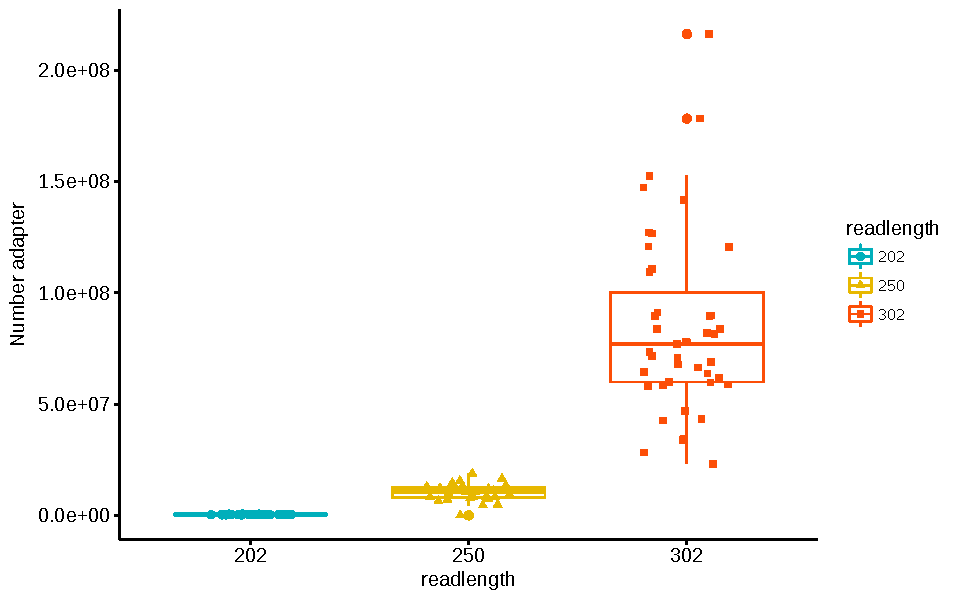
\includegraphics[width=\columnwidth]{./Figures/adapter_contam.pdf}
	\caption{\textbf{Number of detected adapter sequences by length of RNAseq reads:} Total numbers and variance of adapter contamination increases drastic with longer reads. This emphasizes the importance of adapter trimming for reads close to the average length of inserts.}
	\label{fig:adapter_contam}
\end{figure}



\begin{figure}
	\centering
	\begin{subfigure}[t]{0.55\columnwidth}
		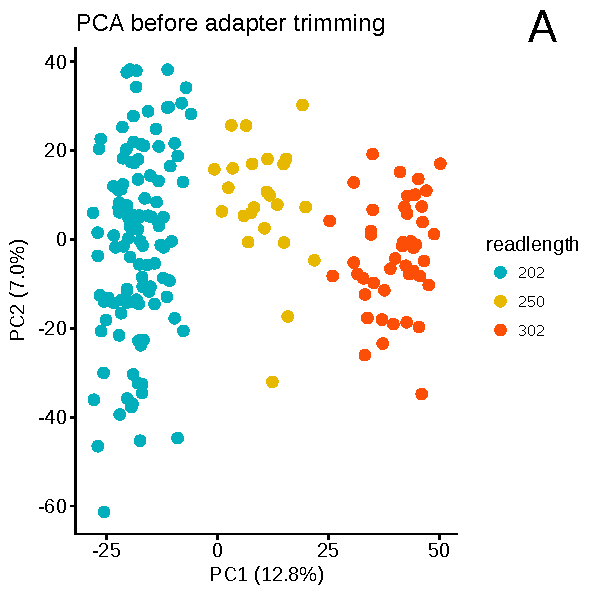
\includegraphics[width=\columnwidth]{./Figures/pca_readlengthOld.pdf}
		\subcaption*{}
		\label{fig:PCA_readlengthOld}
	\end{subfigure}
	\quad
	%add desired spacing between images, e. g. ~,def\svgwidth{\columnwidth} \quad, \qquad, \hfill etc. 
	%(or a blank line to force the subfigure onto a new line)
	\begin{subfigure}[t]{0.6\columnwidth}
		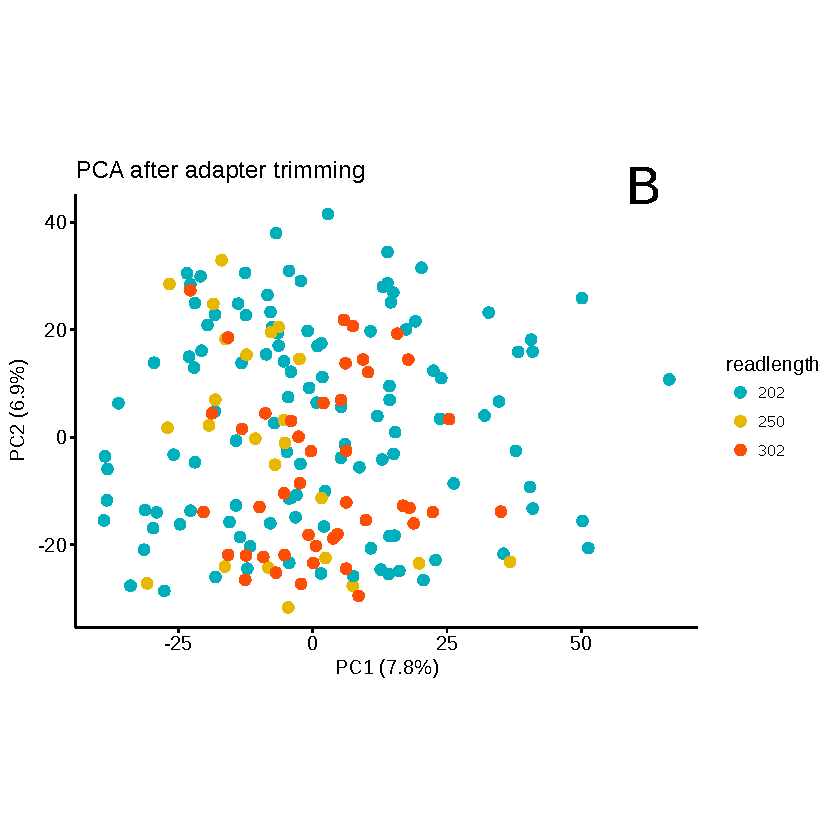
\includegraphics[width=\columnwidth]{./Figures/pca_readlengthtrimmed.pdf}
		\subcaption*{}
		\label{fig:PCA_readlength_trimmed}
	\end{subfigure}
	\caption{\textbf{PCA before and after adapter trimming:} \textbf{(A)} PCA before adapter trimming: The highest variance is associated with the length of RNAseq reads. \textbf{(B)} PCA after adapter trimming: Samples can not longer be distinguished by read length.}
	\label{fig:Trimming}
\end{figure}



\FloatBarrier

\subsubsection{T-cell contamination}
According to exploratory data analysis 7.8\% of variance in PACE transcriptome data were associated to the RNA preparation protocol, which differs in its specificity for B cell selection. To correct for contamination with T cells a variable describing the amount of contamination per sample was introduced and used as co-variable in further gene expression models. T cell marker gene expression showed a gradient between samples, with uniform expression within each sample (Figure \ref{fig:TCell}A). PCA on this marker genes separated sample on PC1 in line with this gradient (Figure \ref{fig:TCell}B). Loadings on PC1 were used to describe the variance of the data set due to T cell contamination.   

\FloatBarrier

\begin{figure}
	\centering
	\begin{subfigure}[t]{\columnwidth}
		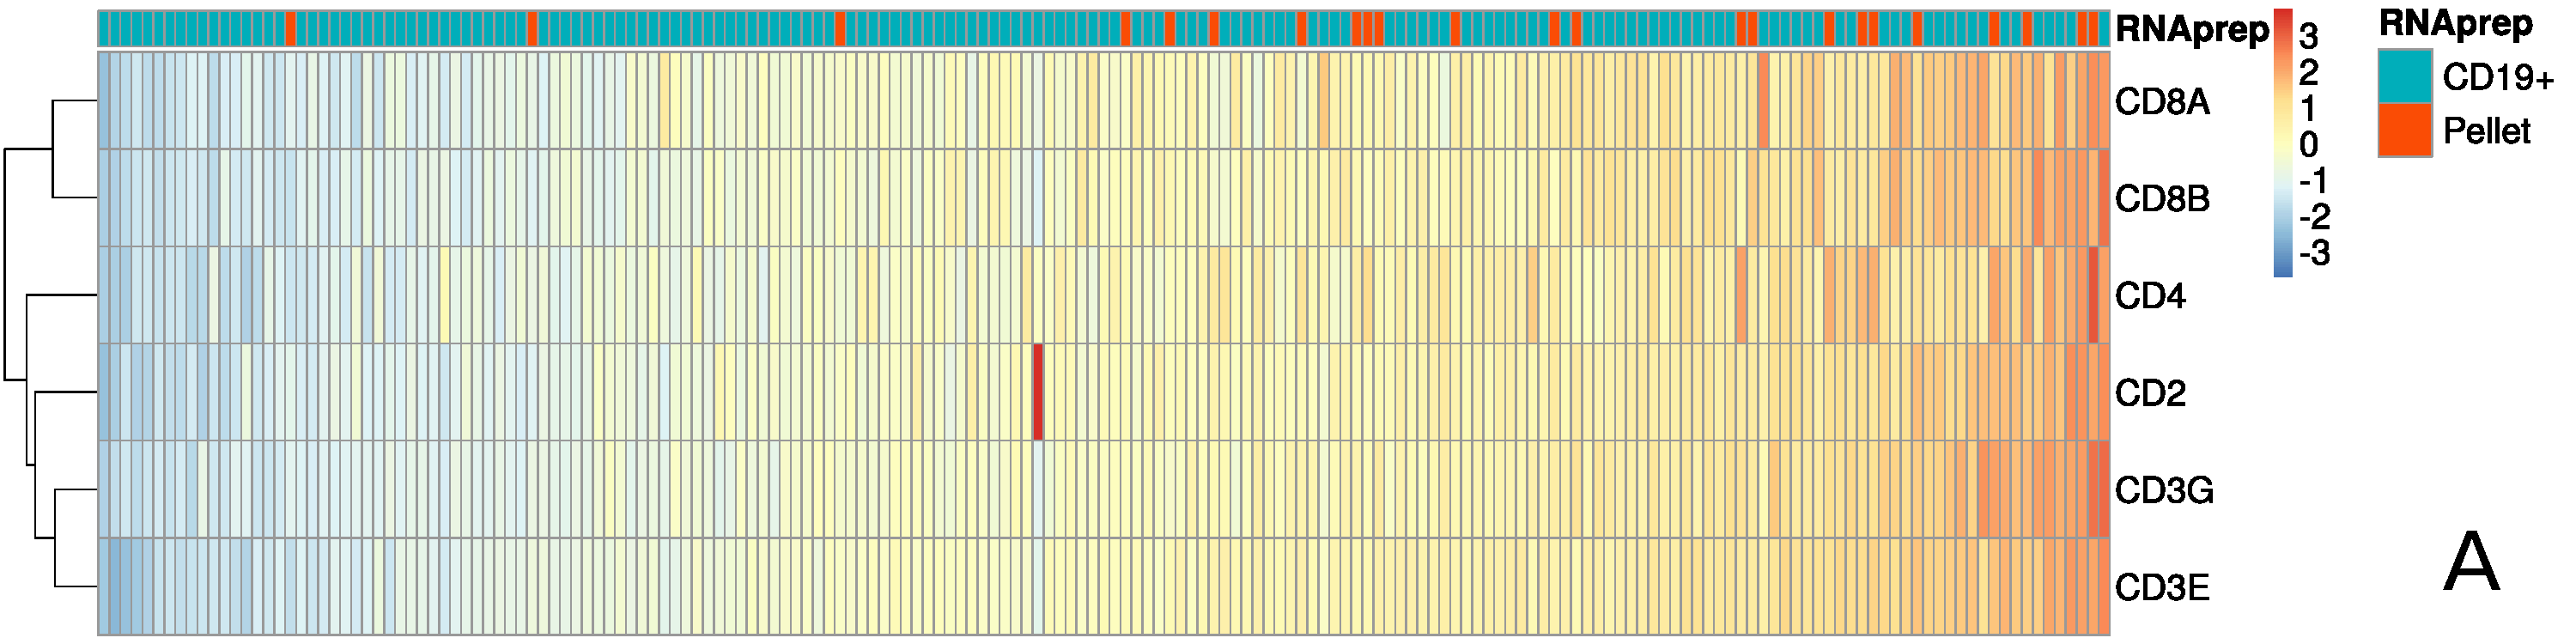
\includegraphics[width=\columnwidth]{./Figures/TmarkExpression.pdf}
		\subcaption*{}
		\label{fig:TmarkExpression}
	\end{subfigure}
	\hfill
	%add desired spacing between images, e. g. ~,def\svgwidth{\columnwidth} \quad, \qquad, \hfill etc. 
	%(or a blank line to force the subfigure onto a new line)
	\begin{subfigure}[t]{\columnwidth}
		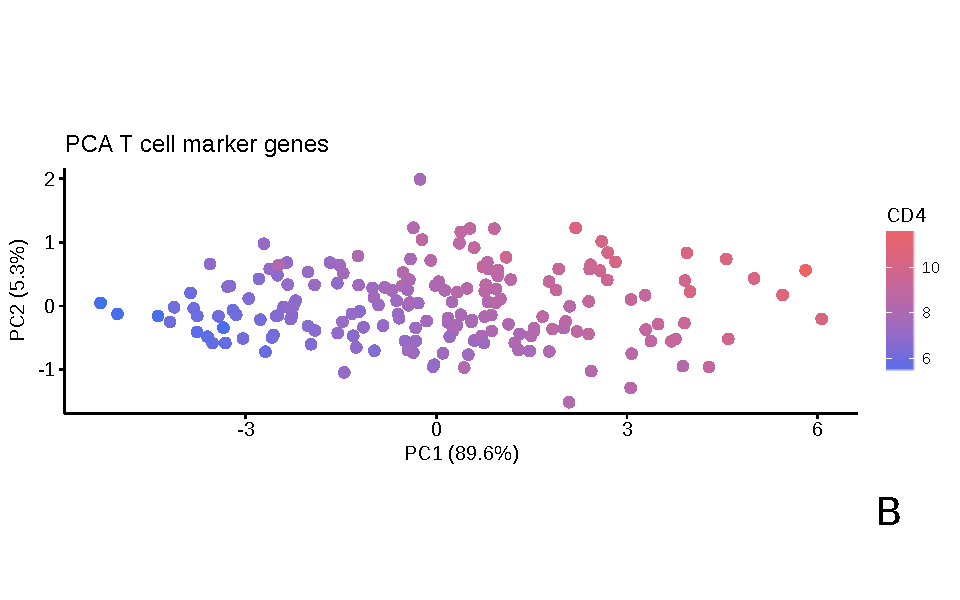
\includegraphics[width=\columnwidth]{./Figures/Tmark_pca.pdf}
		\subcaption*{}
		\label{fig:TmarkPCA}
	\end{subfigure}
	\caption{\textbf{Degree of T cell contamination by marker genes:} \textbf{(A)} T cell marker gene expression show a gradient between samples, with uniform expression within each sample. \textbf{(B)} PC1 describes variance by marker gene expression. Thus loadings were used to quantify T cell contamination.}
	\label{fig:TCell}
\end{figure}

\FloatBarrier



\subsection{Systematic gene Expression Profiling}
Transciptional signatures consist of genes distinguishing variants and were described by differential expressed genes and pathways, that were enriched for them. By integration of other data types and biological knowledge these pattern led to candidates and hypothesis for further investigation.  


\subsubsection{IGHV}
IGHV mutational status is a dominant feature in EDA and resulted in 3873 significant differential expressed genes ($\text{p}_\text{adj} < 0.01$). 92 of them show a $\log_2$ fold change $>4$. These genes could be divided into two groups: those with increased expression in the IGHV-mutated group and those with increased expression in the IGHV-unmutated group, except for Trisomy12 samples. Trisomy12 samples formed a distinct cluster close to the IGHV-mutated cluster. This is internally separated by IGHV status, again indicating interactions between these variants (see Tumor epistatsis). 
In accordance with EDA, methylation groups also clustered by genes distinguishing IGHV groups. Thereby the intermediate group formed a distinct cluster close to the highly methylated group (Figure \ref{fig:gene_exprIGHV_gsea_hallmark}). Marker genes like ZAP-70 and CD38 were higher expressed in IGHV-unmutated samples confirming prior findings. Furthermore SAGE1, which belongs to a class of genes only activated in tumor cells was found in IGHV-unmutated samples. Tumor supressor genes like TP63, TEAD1 and DIRAS3 were also significantly higher expressed. Gene set enrichment analysis revealed B cell receptor signaling as one of the most distinctive changes upon IGHV mutation (Supplements Figure \ref{fig:Enrichment_others}). Using the hallmark gene set annotation revealed a decreased expression of TNF alpha signaling via the NFKB, PI3K-AKT-MTOR pathway and Notch signaling in IGHV-M samples (Figure \ref{fig:EnrichmentTri12IGHV}).  

\FloatBarrier

\begin{figure}
	\centering
	\includegraphics[width=\columnwidth]{./Figures/gene_exprIGHV_gsea_Hallmark.pdf}
	\caption{\textbf{Gene expression of differentially expressed genes by IGHV status:} Samples form distinct cluster depending on IGHV status with Trisomy12 samples forming an own cluster. Genes with $>$ 4.5 $\log_2$ fold change are annotated. Among them are SEPT10, TP63 and TEAD1. Clinical marker ZAP70 and CD38 are up regulated in IGHV unmutated samples.}
	\label{fig:gene_exprIGHV_gsea_hallmark}
\end{figure}


\FloatBarrier

\subsubsection{Trisomy12} 
Trisomy12 is a common genetic variant in CLL samples. On gene expression level we found 3942 differentially expressed genes ($\text{p}_\text{adj} < 0.01$), which formed two major cluster of up and down regulated genes in Trisomy 12 (Figure \ref{fig:gene_exprTriisomy12_gsea_hallmark}). In line with expectations most up regulated genes ($\sim22\%$) were located on chromosome 12 (Figure \ref{fig:tri12_chrom}). Among up regulated genes, we found surface integrins like ITGAM, ITGB2, ITGB1 and ITGB7 and integrin signaling molecules associated with VLA-4 directed adhesion. Similar to the IGHV unmutated group, up regulated genes were enriched in TNF alpha signaling via NFKB, PI3K-AKT-MTOR signaling, Notch signaling and P53. In contrast, down regulated genes were associated with bile acid metabolism and glycolysis (Figure \ref{fig:EnrichmentTri12IGHV}B). 

\FloatBarrier

\begin{figure}
	\centering
	\includegraphics[width=\columnwidth]{./Figures/gene_exprTrisomy12_gsea_Hallmark.pdf}
	\caption{\textbf{Gene expression in Trisomy12:} Trisomy12 samples form a separate cluster with distinct gene expression. Genes with $\log_2$ fold changes $>4.5$ are annotated. Among them surface integrins like ITGAM, ITGB2, ITGB1 and ITGB7 can be found. Many up regulated genes are located on chromosome 12.}
	\label{fig:gene_exprTriisomy12_gsea_hallmark}
\end{figure}


\begin{figure}
	\centering
	\begin{subfigure}[t]{0.48\columnwidth}
		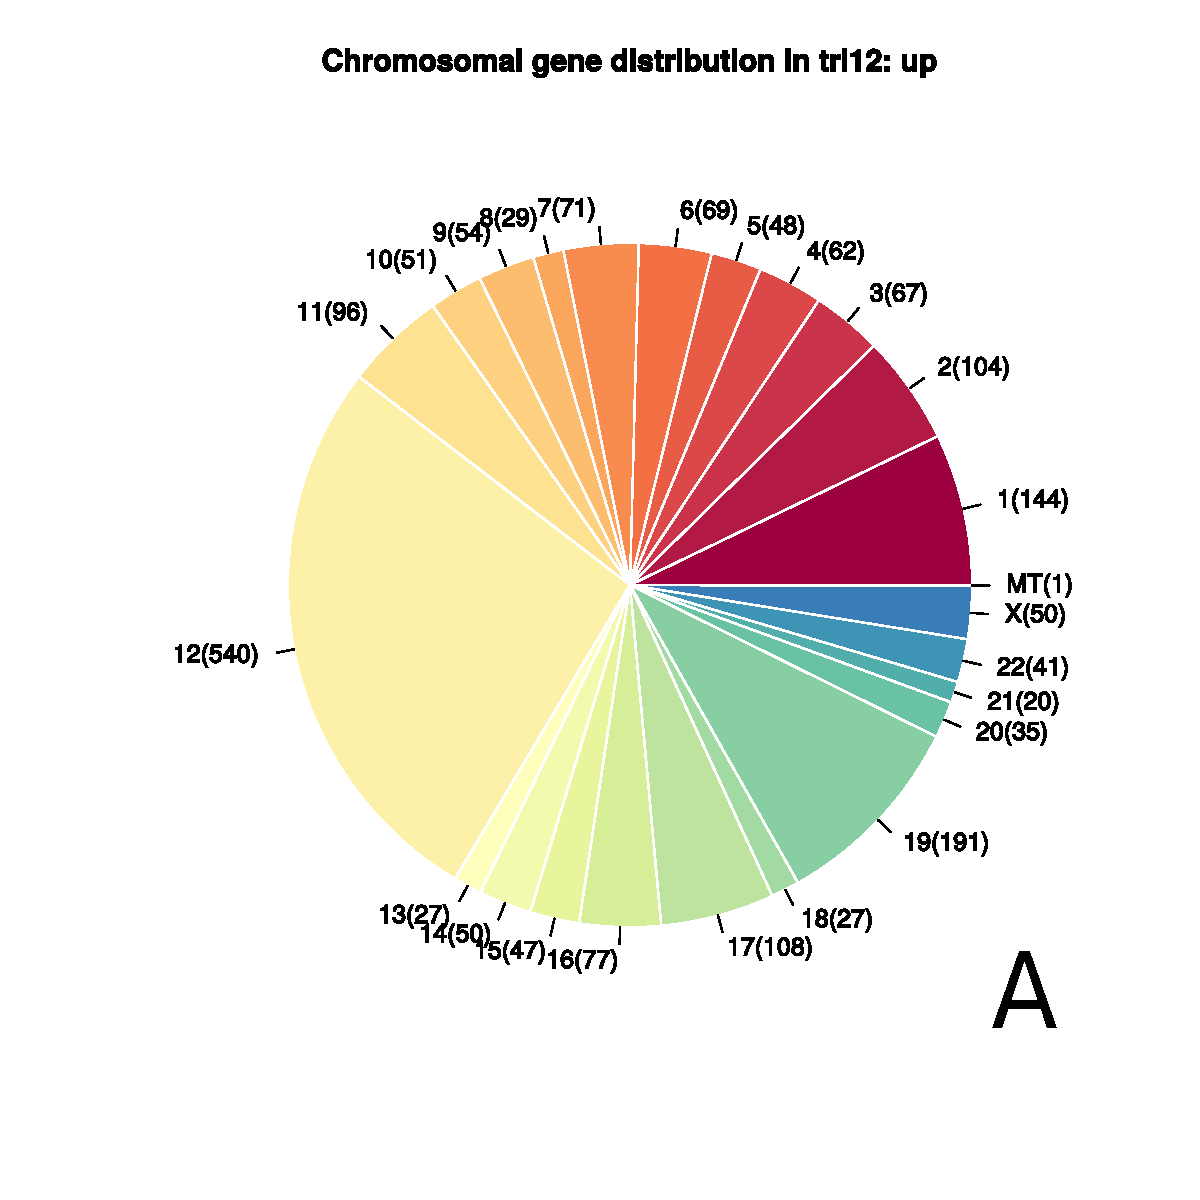
\includegraphics[width=\columnwidth]{./Figures/chromosom_dist_up.pdf}
		\subcaption*{}
		\label{fig:tri12_chrom_dn}
	\end{subfigure}
	\hfill
	%add desired spacing between images, e. g. ~,def\svgwidth{\columnwidth} \quad, \qquad, \hfill etc. 
	%(or a blank line to force the subfigure onto a new line)
	\begin{subfigure}[t]{0.48\columnwidth}
		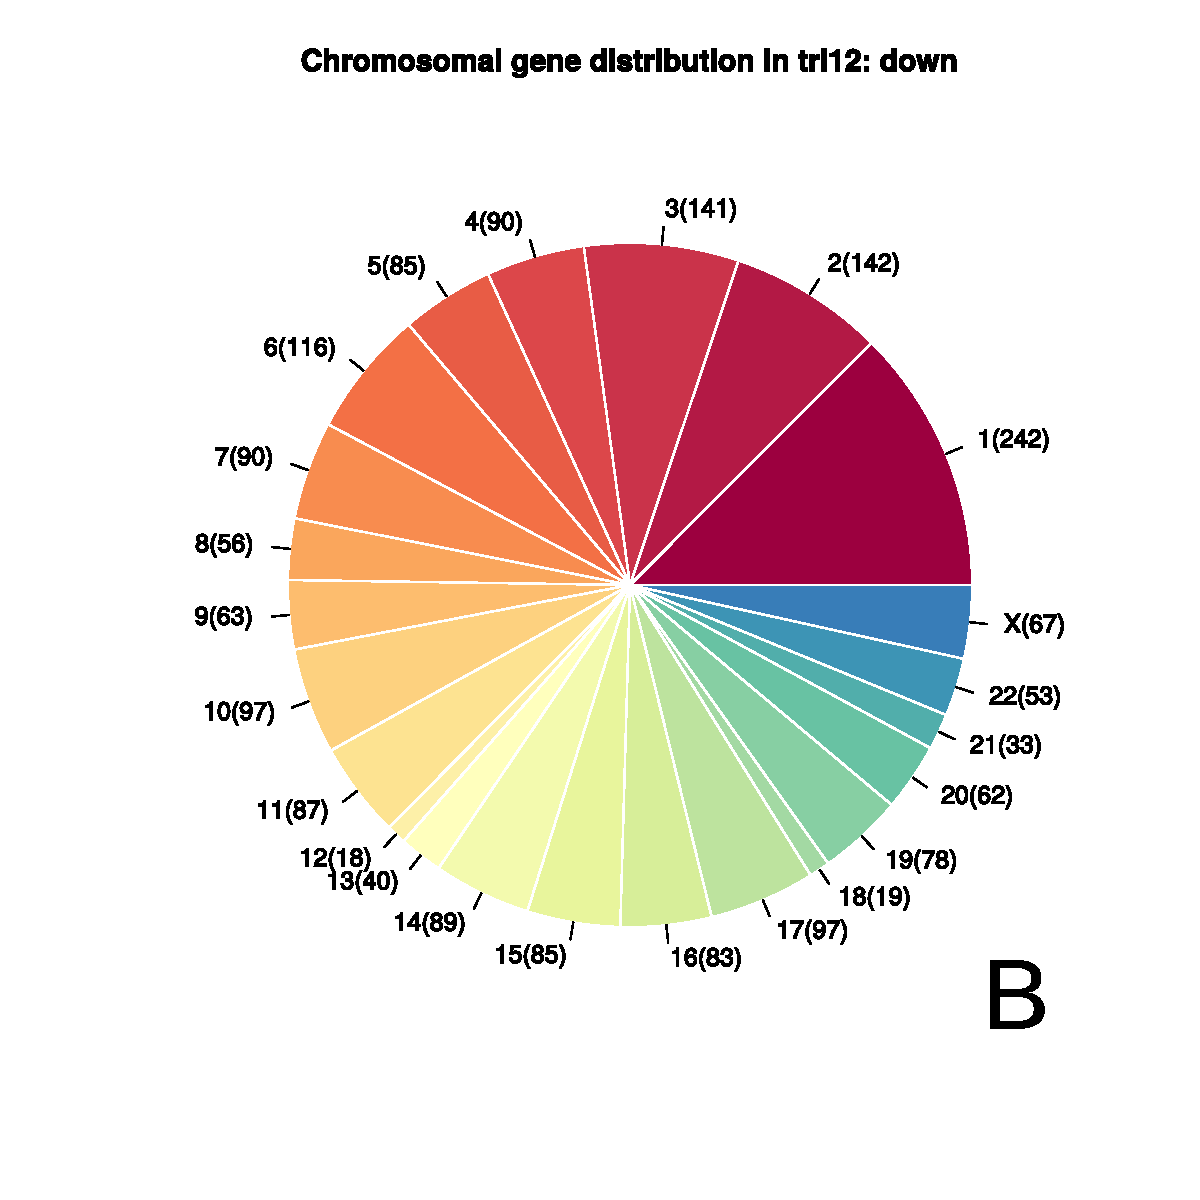
\includegraphics[width=\columnwidth]{./Figures/chromosom_dist_down.pdf}
		\subcaption*{}
		\label{fig:tri12_chrom_up}
	\end{subfigure}
	\caption{\textbf{Chromosomal distribution of genes differentially expressed in Trisomy12 samples:} \textbf{(A)} 22\% of up regulated genes are located on chromosome 12. Numbers in captions indicate the number of differentially expressed genes located at this chromosome. \textbf{(B)} 
		Genes down regulated in Trisomy12 samples are approximately equally distributed among chromosomes.}
	\label{fig:tri12_chrom}
\end{figure}


\begin{figure}
	\centering
	\begin{subfigure}[t]{0.48\columnwidth}
		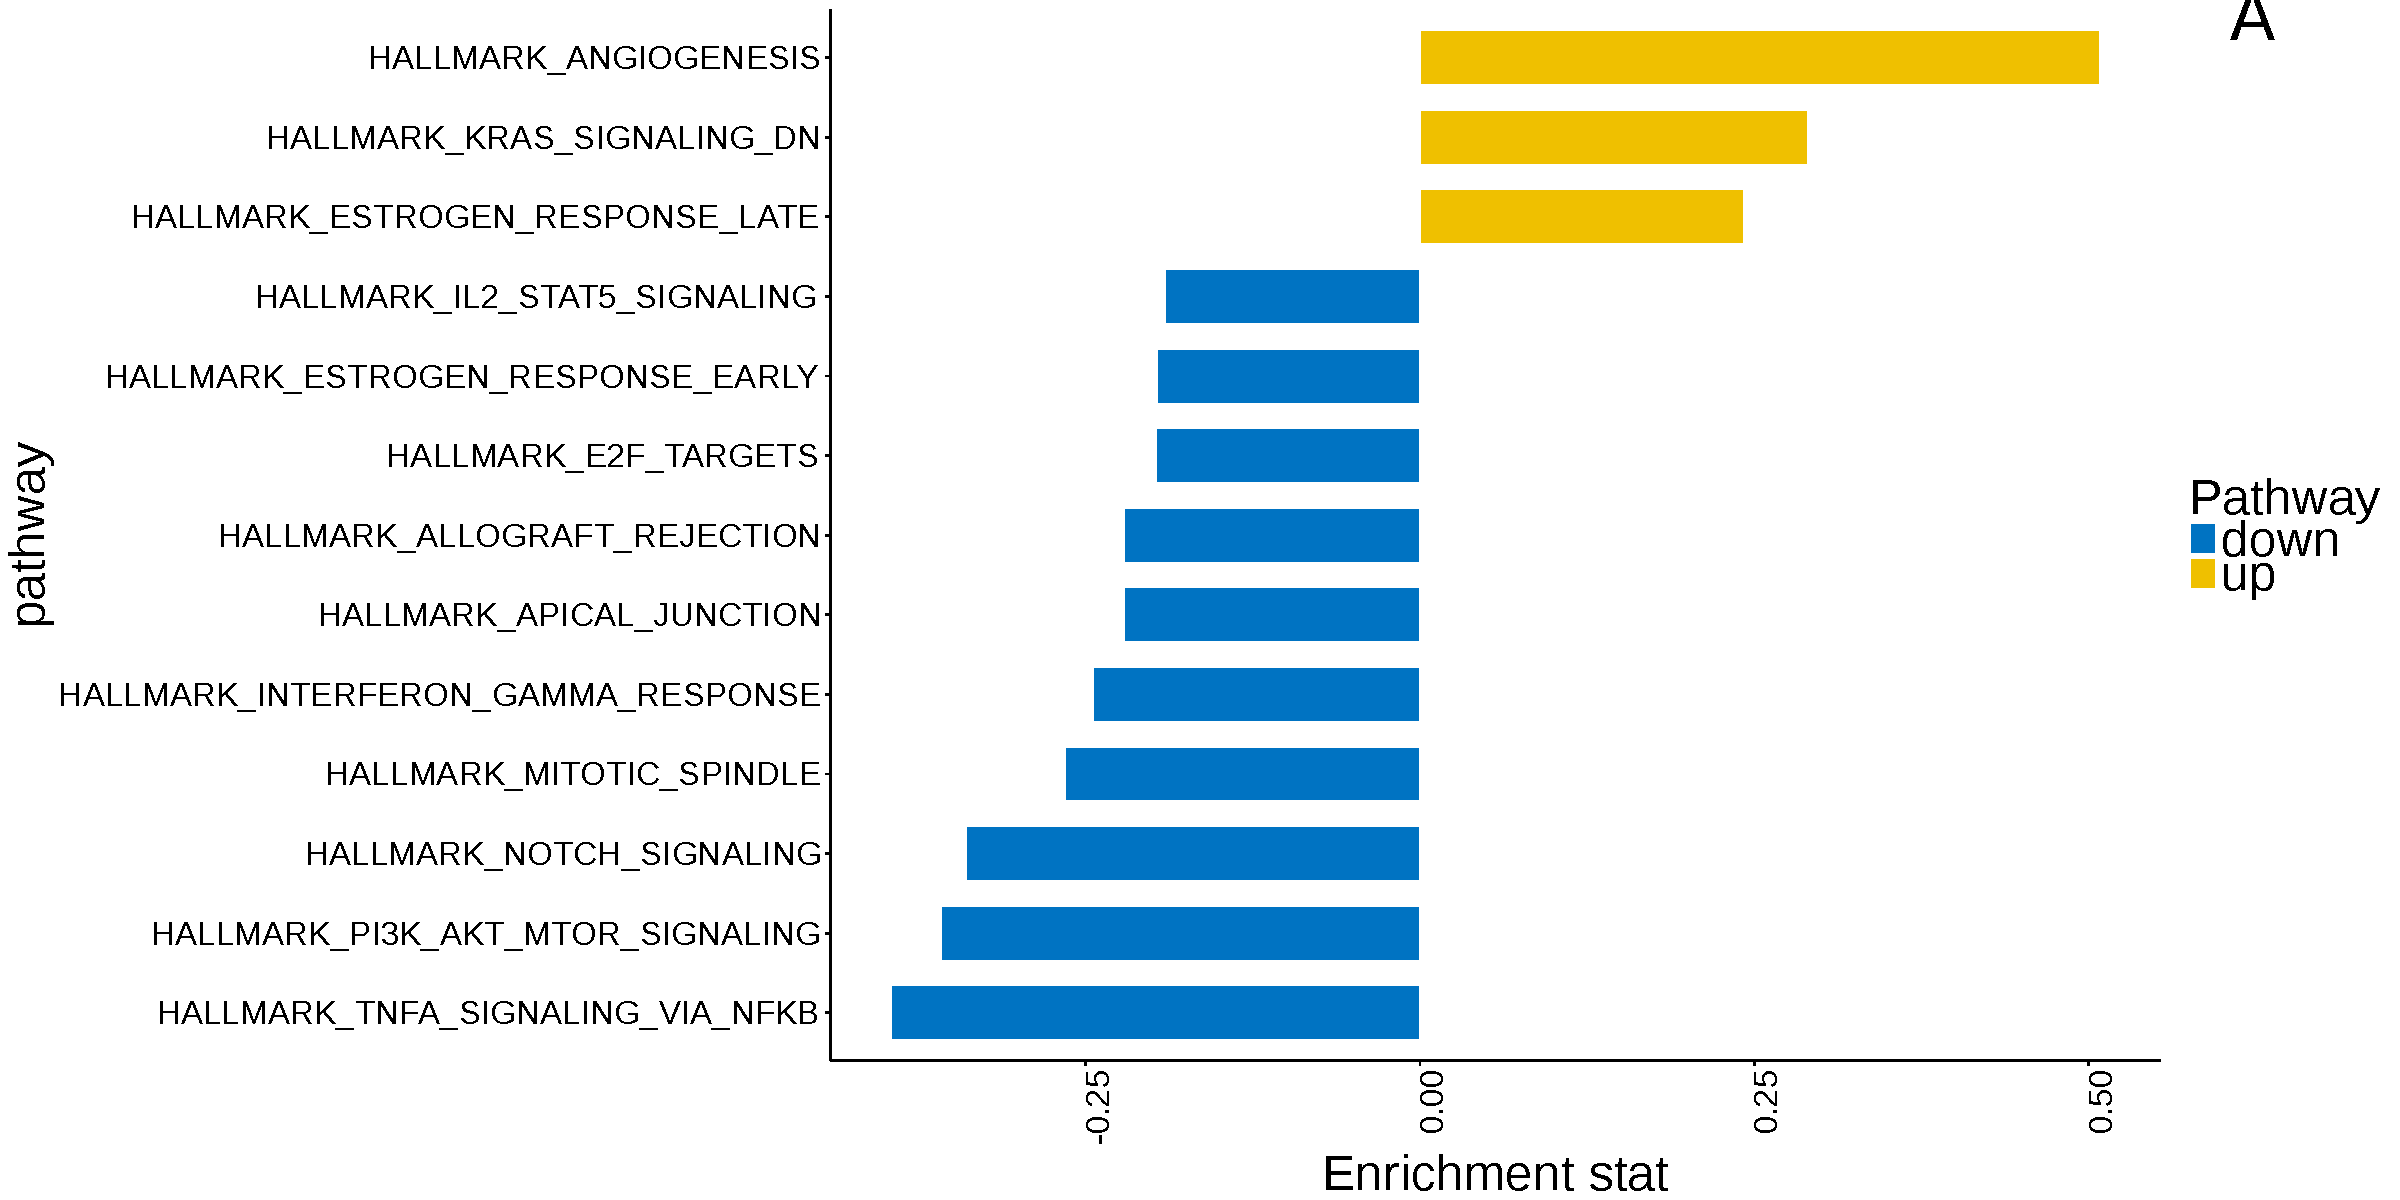
\includegraphics[width=\columnwidth]{./Figures/gsea_IGHV.pdf}
		\subcaption*{}
		\label{fig:gsea_IGHV}
	\end{subfigure}
	\hfill
	%add desired spacing between images, e. g. ~,def\svgwidth{\columnwidth} \quad, \qquad, \hfill etc. 
	%(or a blank line to force the subfigure onto a new line)
	\begin{subfigure}[t]{0.48\columnwidth}
		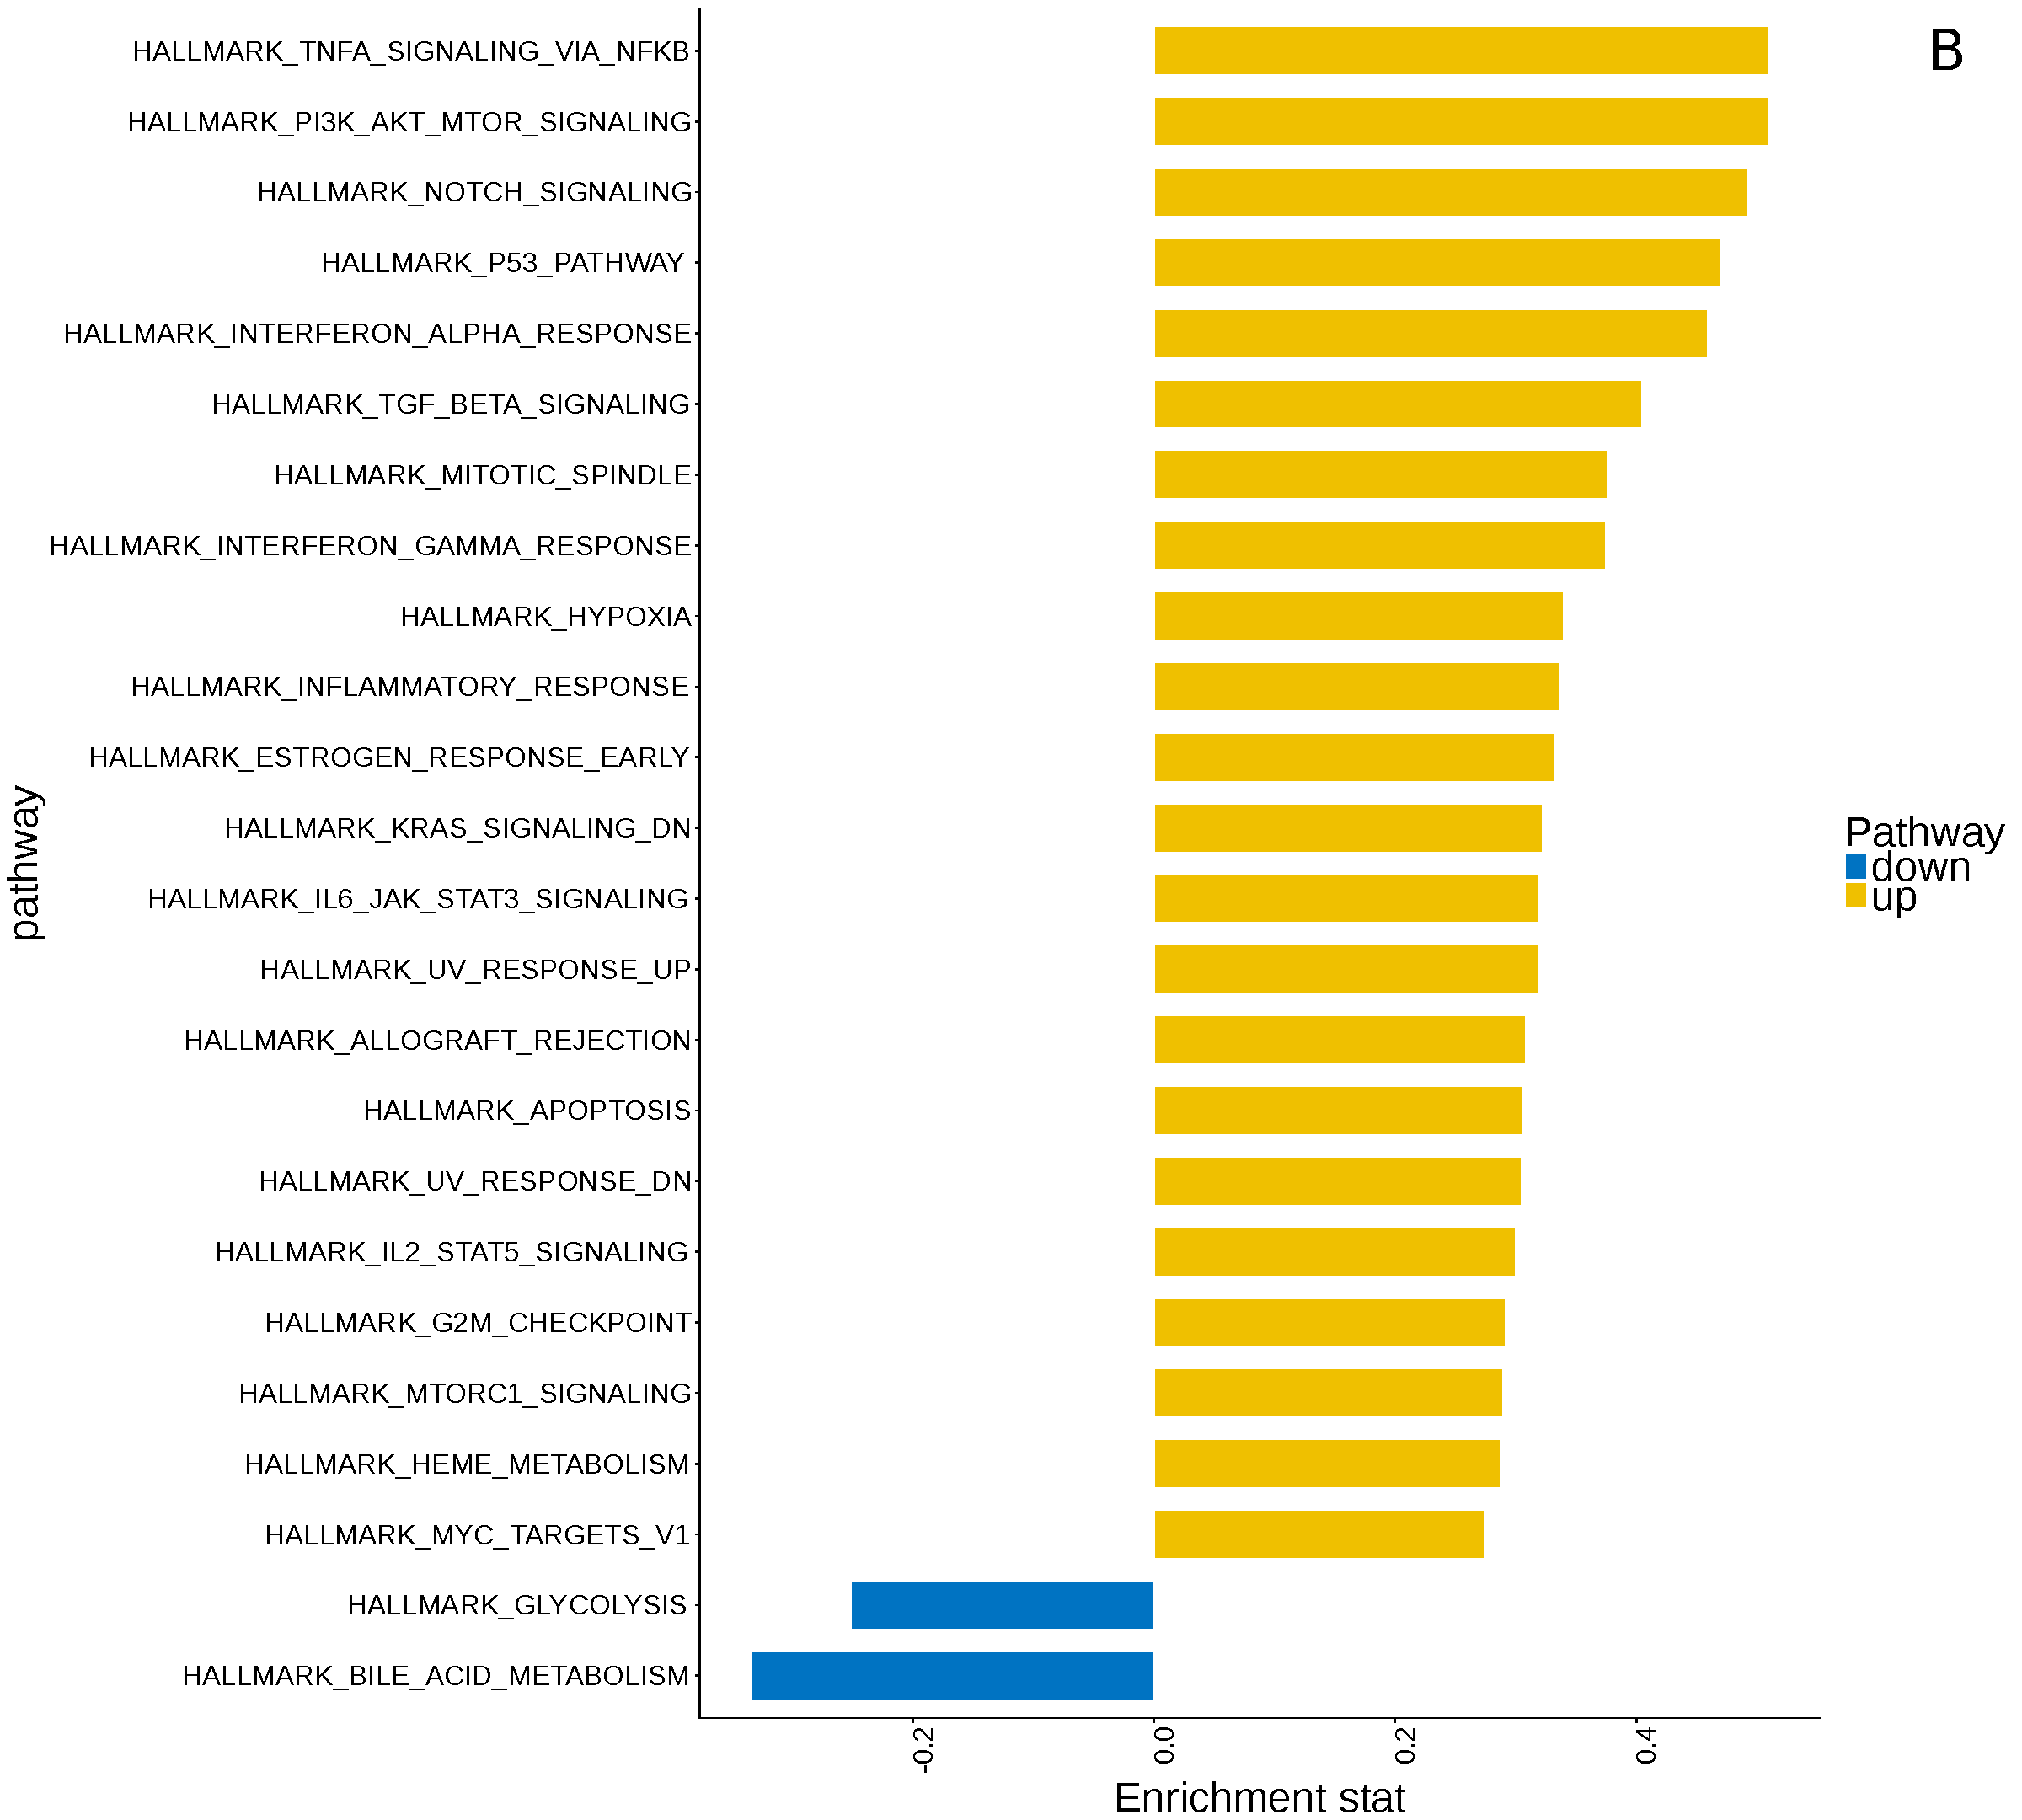
\includegraphics[width=\columnwidth]{./Figures/gseaHallmark_trisomy12.pdf}
		\subcaption*{}
		\label{fig:gsea_trisomy12}
	\end{subfigure}
	\caption{\textbf{Enriched hallmark gene sets:} \textbf{(A)} Enriched pathways in IGHV samples are shown. Up regulated pathway as angiogenesis are higher expressed in IGHV-mutated samples. Down regulated pathways in IGHV mutated vs unmutated samples are TNF alpha signaling via NFKB and PI3 MAP Kinase pathway. \textbf{(B)} Trisomy12 activates many pathways like TNFA via NFKP, Notch pathway and PI3 MAP Kinase pathway.}
	\label{fig:EnrichmentTri12IGHV}
\end{figure}

\FloatBarrier


\subsubsection{TP53 and Del17p53}
The TP53 gene is located at the locus of Del17p13. Thus TP53 mutation in combination with Del17p13 lead to a homozygote loss of function for TP53, which is a regulator of DNA damage response. More than half of all samples with Del17p13 were found to have a mutated TP53 gene at the other allel. Gene signatures of mutation and deletion were dominated by down regulated genes on chromosome 17 (Figure \ref{fig:gene_exprdel17p13_gsea_kegg}). Patterns of up regulated genes were less distinct. All in all 929 genes were differentially expressed in Del17p13 samples and 474 in TP53 samples ($\text{p}_\text{adj} < 0.01$). Half of those were overlapping with Del17p13 (Figure \ref{fig:GeneDist17}). TP53 itself was down regulated and clustered with other genes on chromosome 17. Most of Del17p13 and TP53 samples formed one distinct cluster with a correlated expression signature. A few samples showed distinct differences in gene expression, even for down regulated genes on chromosome 17. They seemed to be dominated by another mechanism independent of TP53 and genes on chromosome 17. Enrichment tests revealed DNA repair pathway down regulated in TP53 samples. This is in line with the function of TP53 for DNA damage control. Furthermore both variants are associated with down regulation in Wnt Beta Catenin signaling.   

\FloatBarrier

\begin{figure}
	\centering
	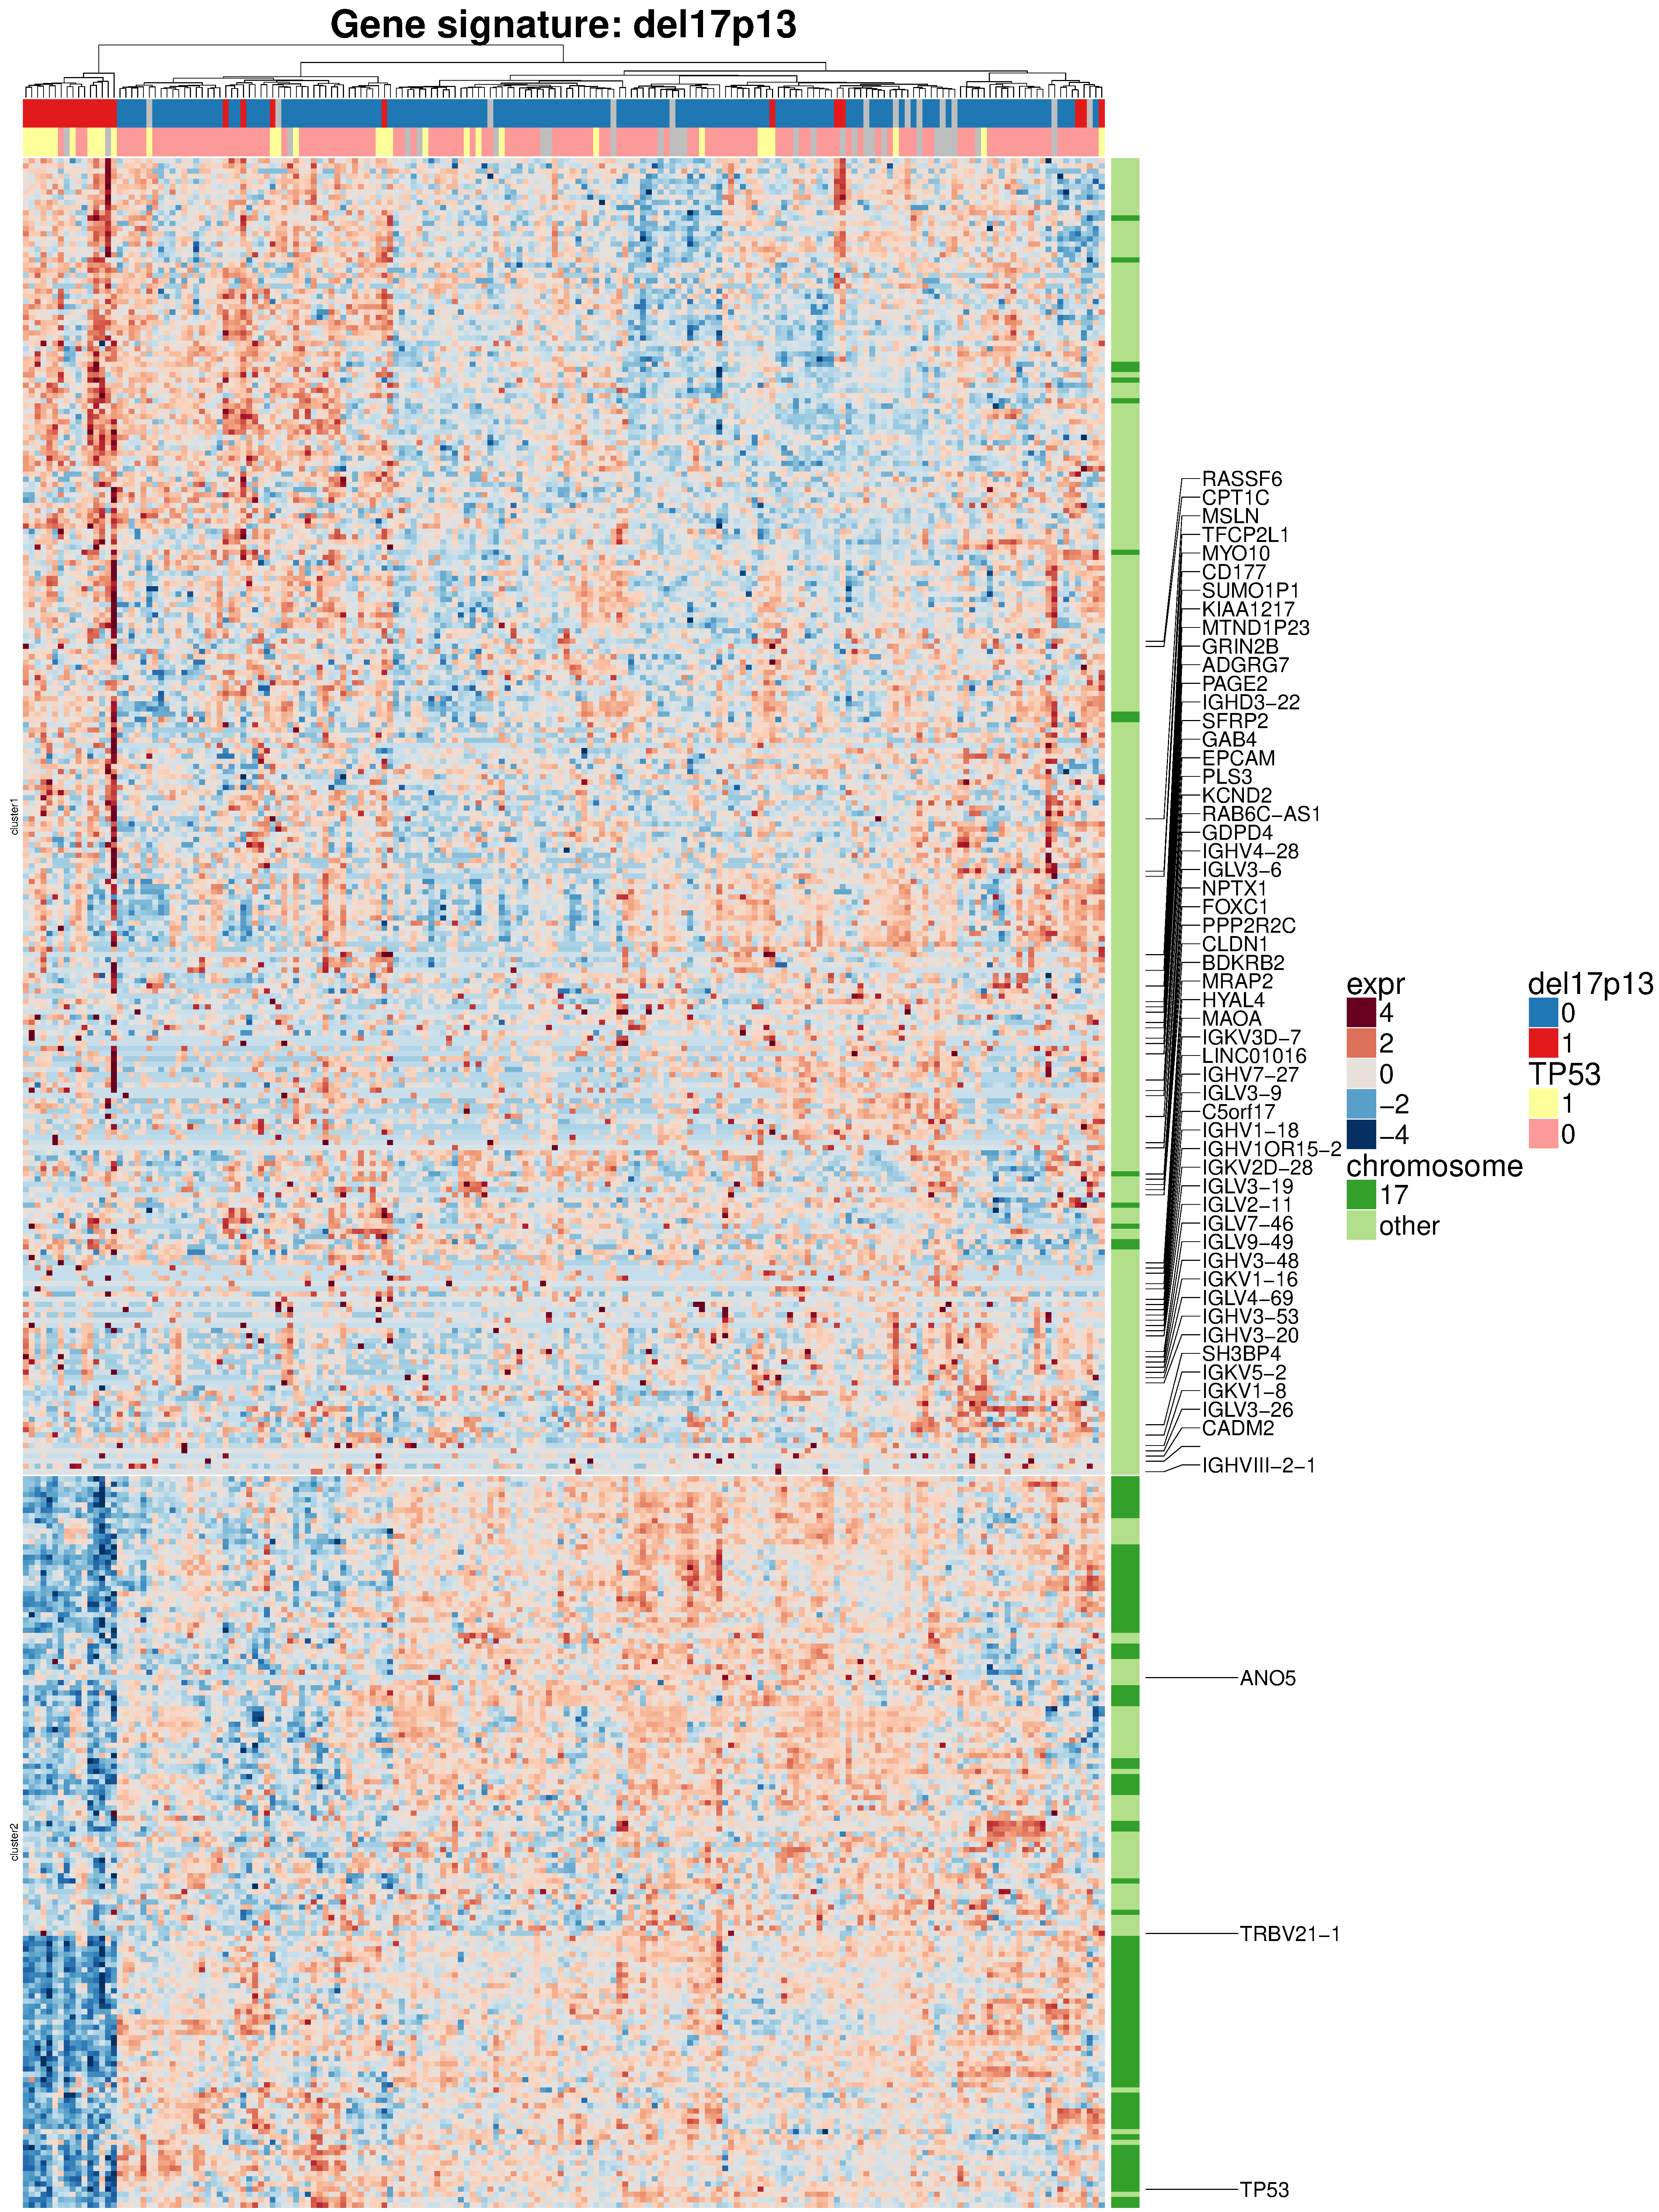
\includegraphics[width=\columnwidth]{./Figures/gene_exprDel17p13_gsea_Kegg.pdf}
	\caption{\textbf{Gene expression in Del17p13 and TP53:} Del17p13 samples cluster together with a few exceptions. Most of these exceptions do not show a TP53 mutation and thus not a complete loss of TP53 function. The cluster is driven by down regulated genes (most located on chromosome 17) including TP53.}
	\label{fig:gene_exprdel17p13_gsea_kegg}
\end{figure}

\begin{figure}
	\centering
	\begin{subfigure}[t]{0.8\columnwidth}
		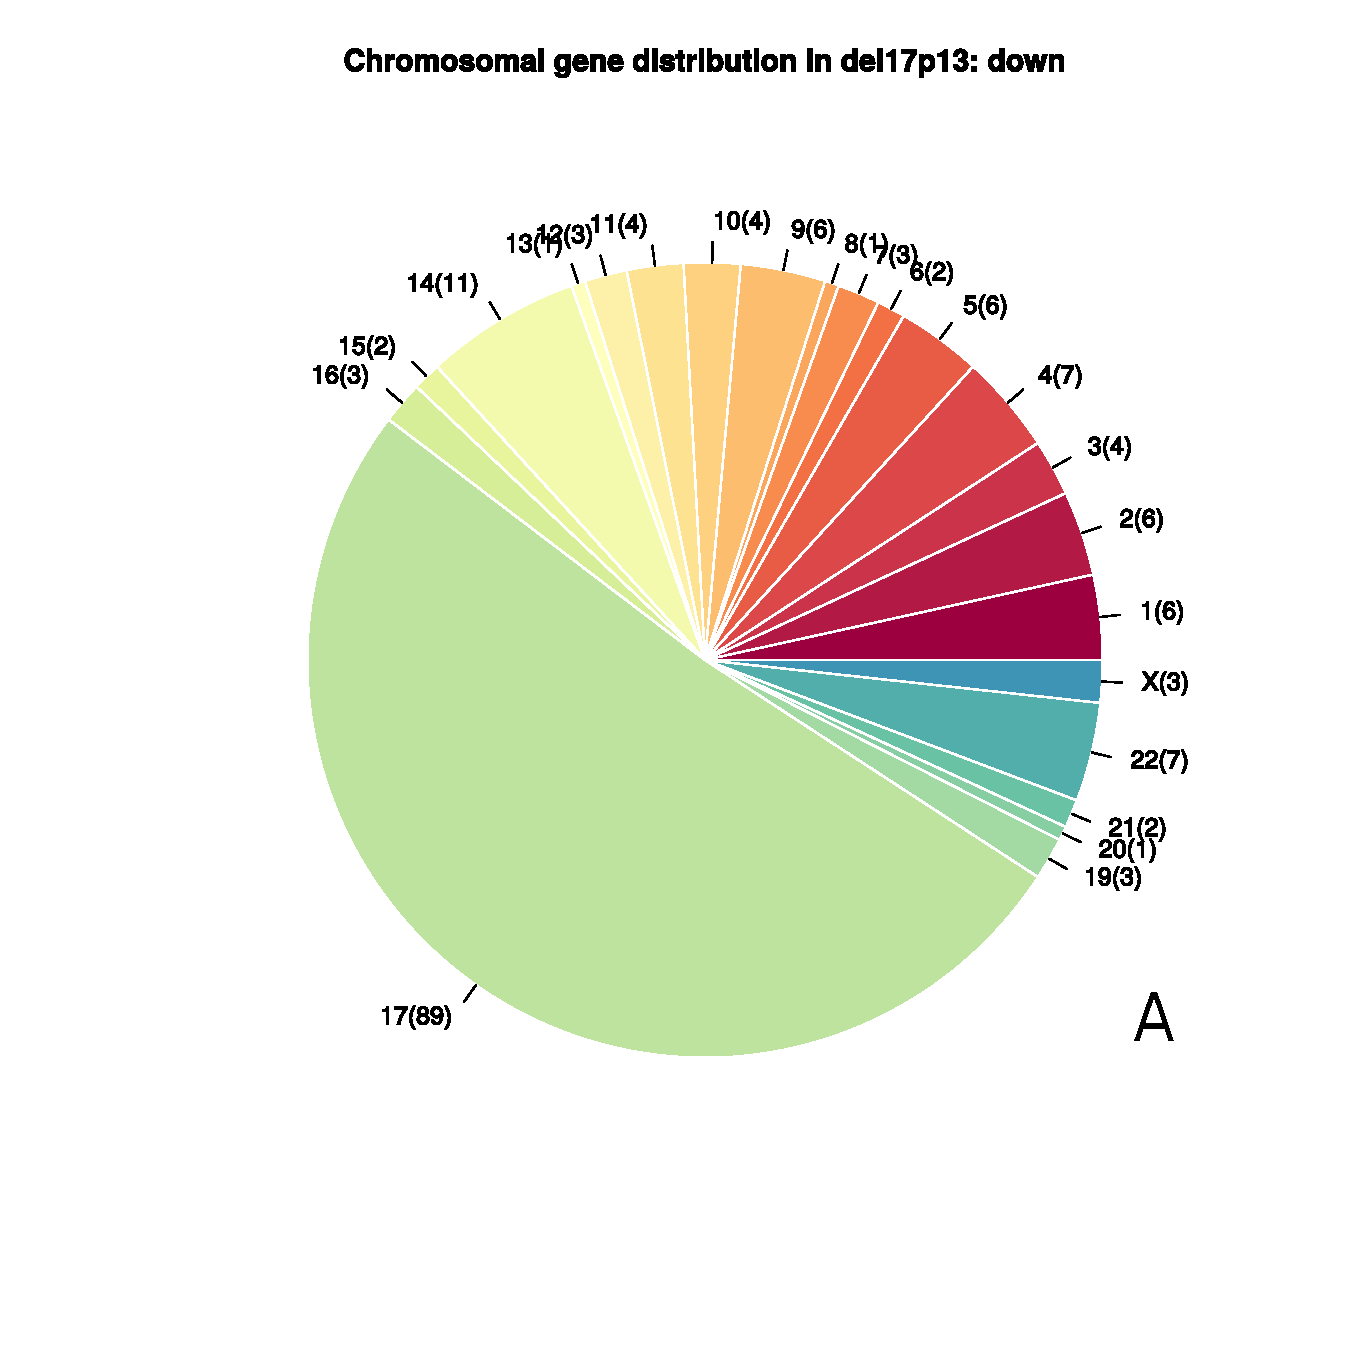
\includegraphics[width=\columnwidth]{./Figures/chromosom17_dist_down.pdf}
		\subcaption*{}
		\label{fig:chromosom17_dist_down}
	\end{subfigure}
	\quad
	%add desired spacing between images, e. g. ~,def\svgwidth{\columnwidth} \quad, \qquad, \hfill etc. 
	%(or a blank line to force the subfigure onto a new line)
	\begin{subfigure}[t]{0.6\columnwidth}
		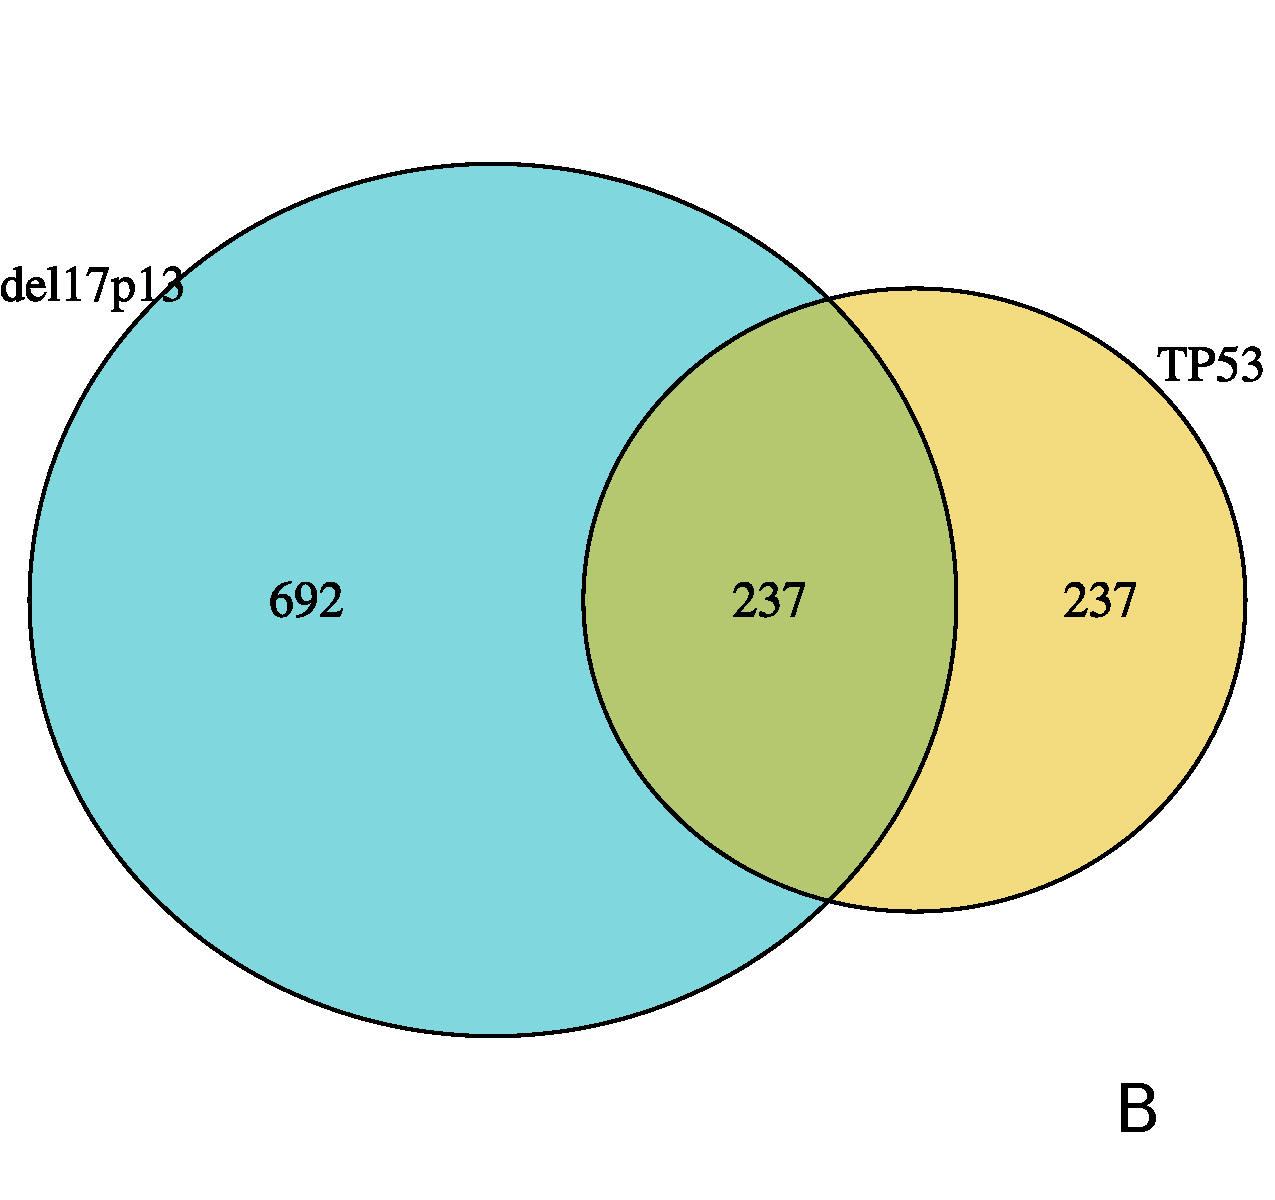
\includegraphics[width=\columnwidth]{./Figures/vennDel17TP53.pdf}
		\subcaption*{}
		\label{fig:vennDel17TP53}
	\end{subfigure}
	\caption{\textbf{Distribution of differentially expressed genes in TP53 and Del17p13} \textbf{(A)} More than half of all down regulated genes in Del17p13 samples are located on chromosome 17. Numbers in captions indicate the number of differentially expressed genes located at this chromosome. \textbf{(B)} There is a high overlap of differentially expressed genes in TP53 and Del17p13.}
	\label{fig:GeneDist17}
\end{figure}


\FloatBarrier

\subsubsection{Del11q22.3 and ATM}
Del11q22.3 is another common deletion in CLL samples. Analysis revealed 430 significantly differential expressed genes ($\text{p}_\text{adj} < 0.05$). About half of them were down regulated and 30.5\% were located on chromosome 11. With some exception Del11.22.3 samples formed a distinct cluster with common gene expression pattern of down regulated as well as up regulated genes (Figure \ref{fig:gene_exprdel11q22.3_gsea_hallmark}). Up regulated pathways were myogenisis, Myc targets and heme metabolism, whereas protein secretion and mitotic spindle were down regulated (see supplements Figure \ref{fig:Enrichment_others}B). The ATM gene is localized on chromosome 11q22 and more than half of all samples with ATM mutation (13 cases in total) had a deletion on the second chromosome. A specific signature for ATM mutation alone or for homozygotic ATM loss of function was not identified, but ATM was among differentially down regulated genes in Del11q22 samples.  

\FloatBarrier

\begin{figure}
	\centering
	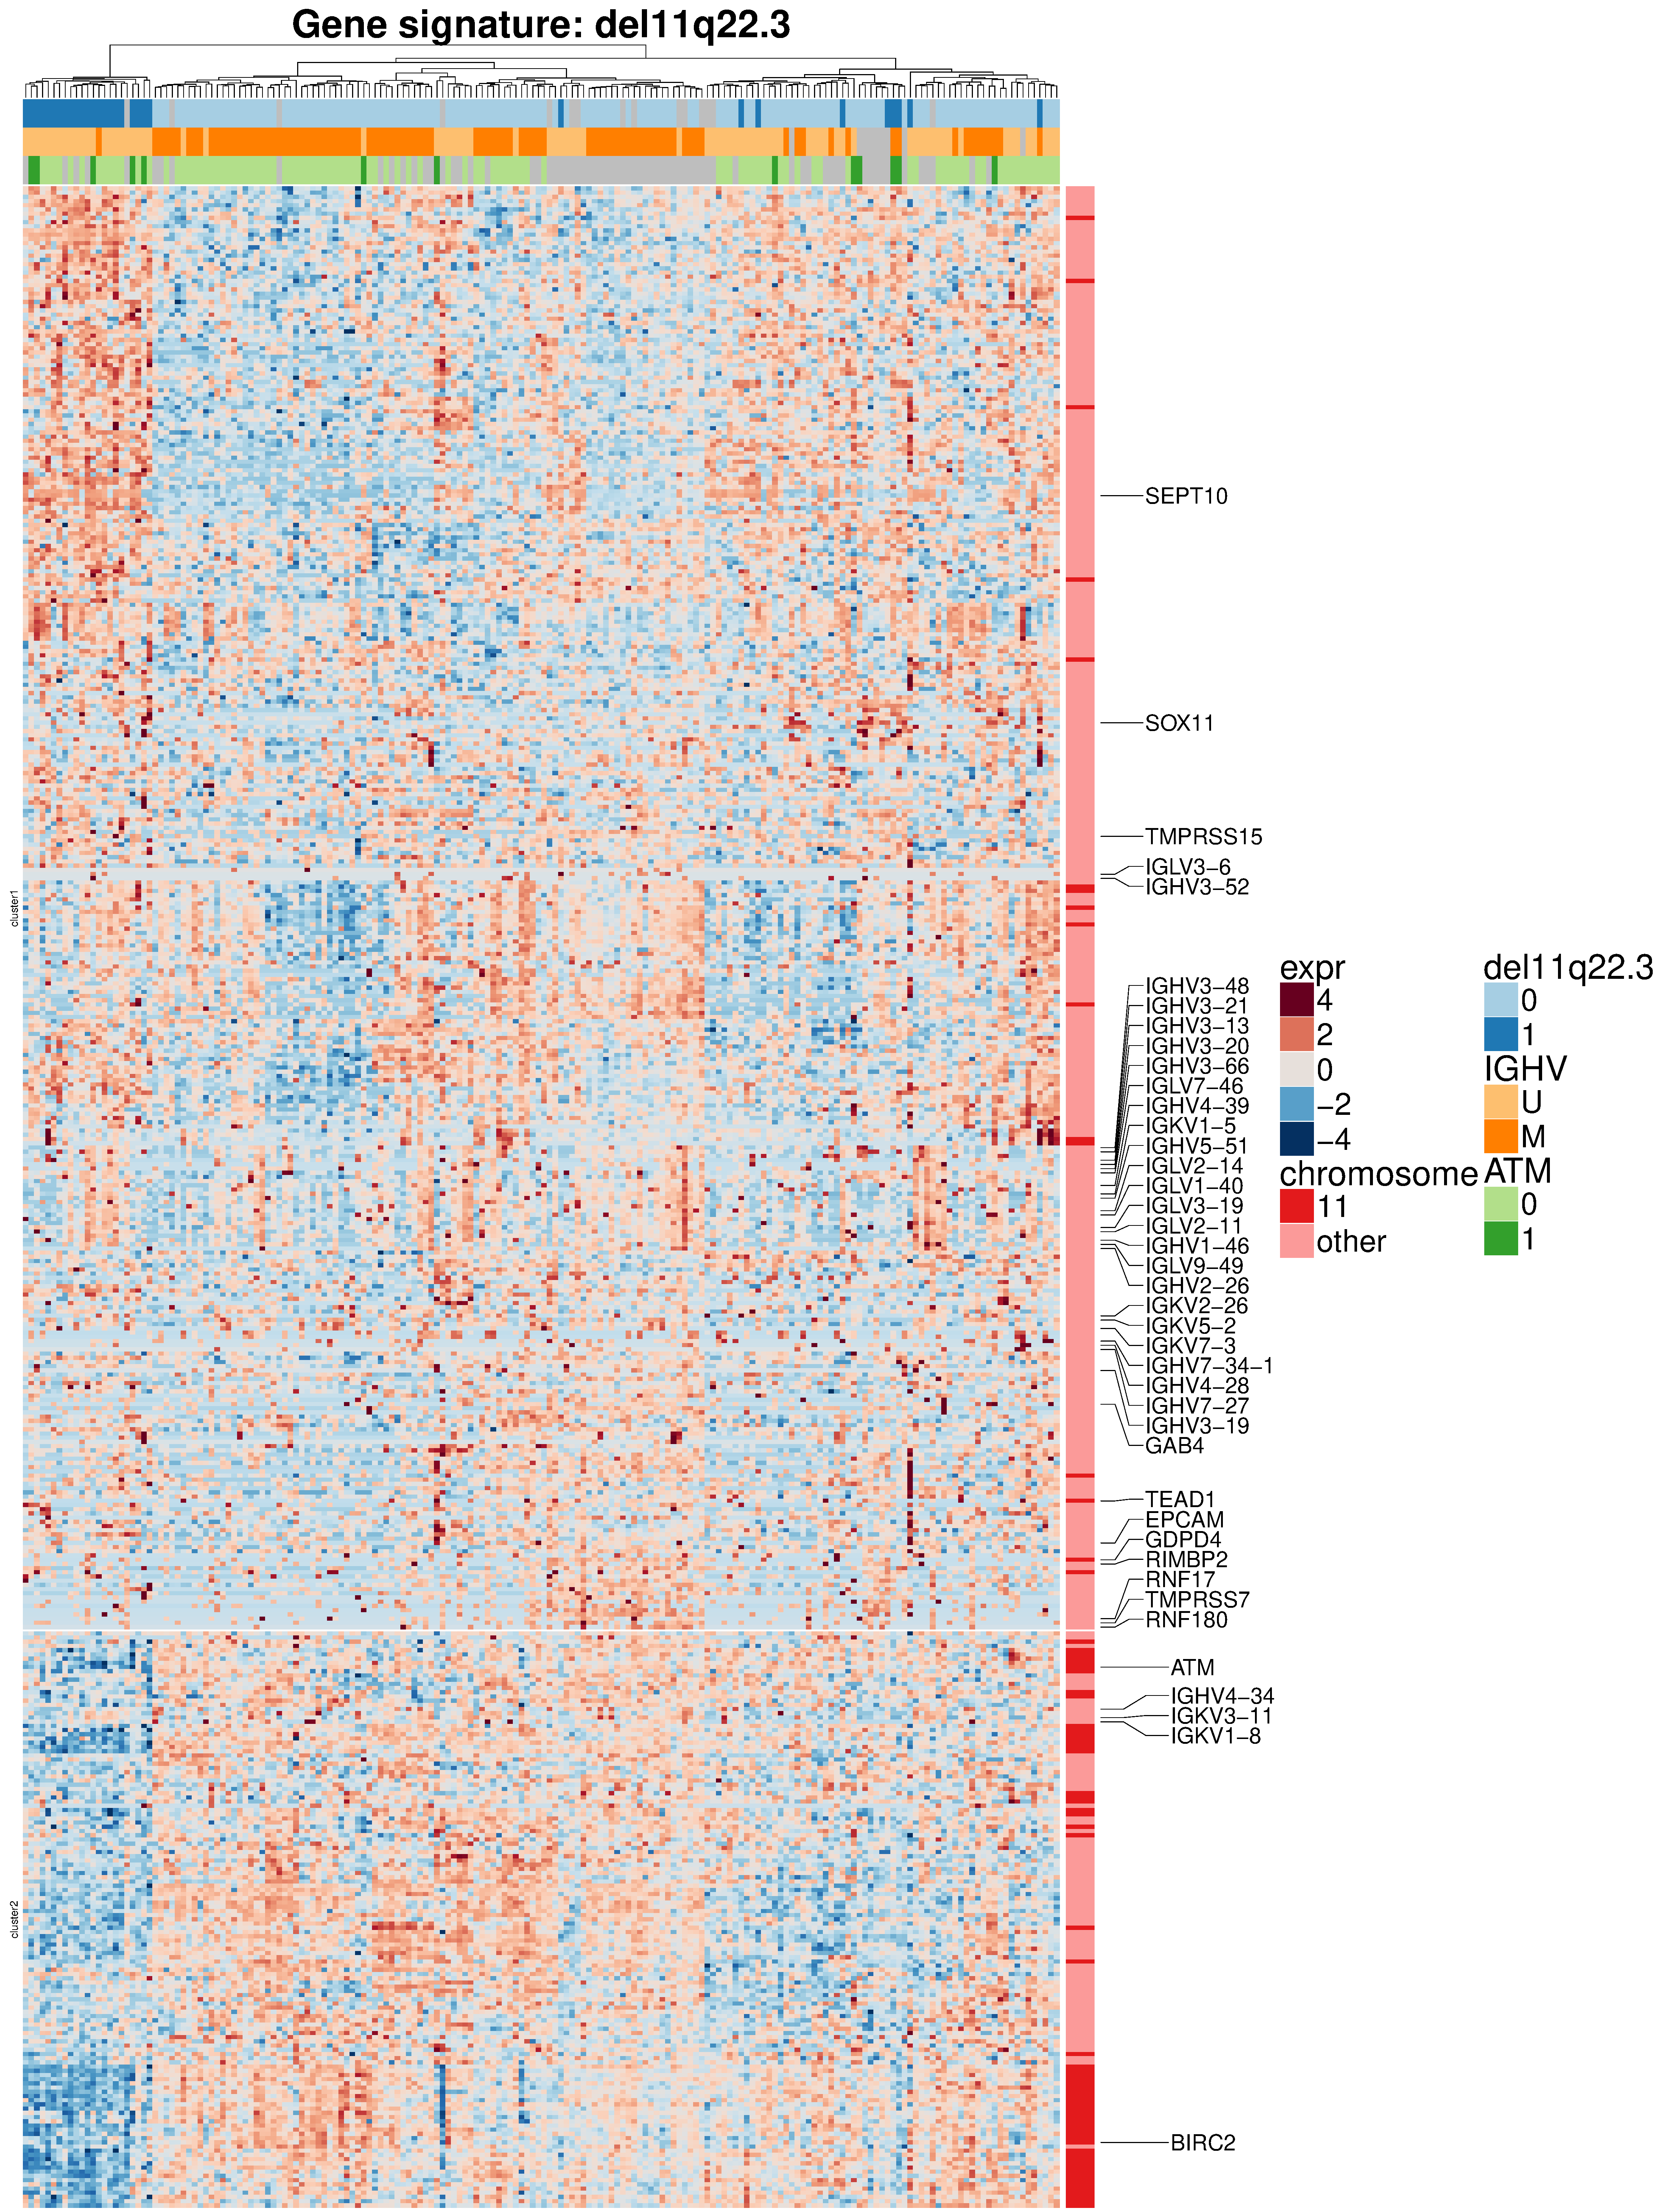
\includegraphics[width=\columnwidth]{./Figures/gene_exprdel11q22_gsea_Hallmark.pdf}
	\caption{\textbf{Gene expression in Del11q22.3 and ATM:} Del11q22 samples cluster driven by deleted genes on chromosome 11 like ATM. Nevertheless loss of ATM function does not seem to be the only driving factor, but a set of genes including SEPT10 is also up regulated.}
	\label{fig:gene_exprdel11q22.3_gsea_hallmark}
\end{figure}

\FloatBarrier



\subsubsection{Del13q14}
Del13q14 is the most common CNV in PACE. Nonetheless the degree of deletion varies a lot between a loss of 100\% and 0\%. On gene expression level the degree of Del13q14 did not correlate with expression pattern at all (see Supplements Figure \ref{fig:gene_exprdel13q14_gsea_kegg}). No pathways were significantly enriched for differentially expressed genes either. A subgroup of samples showed distinct down regulation of a small set of genes that were located at 13q14, including KPNA3, DLEU1, KCNRG, PHF11. Thereby the subgroup itself could not be distinguished by Del13q14 status. Genes from the minimal deleted region like DLEU2, miR15a/16a and genes regulated by the mir15a-mir16a complex like BCL2 were not differentially expressed. Major tumor progressive effects of Del13q14 does not seem to be displayed at gene expression level. 

\subsubsection{Del8p12 and Gain8q24}
More than half of all samples with Gain8q24 show an earlier deletion Del8p12 as genetic instability on chromosome 8. Thus, Del8p12 and Gain8q24 samples showed both, significantly up- and down regulated genes on chromosome 8. In total 206 resp 285 genes were differentially expressed and enriched in similar pathways (Figure \ref{fig:gene_exprgain8q24_gsea_Hallmark}). Unfolded protein response, mTORC1 signaling and Myc targets were up and myogenesis was significantly down regulated (see Supplements Figure \ref{fig:Enrichment_others}C). Enrichment in Myc targets was in line with prior findings and has been proposed as possible mechanism of Gain8q24 tumorigenesis.

\FloatBarrier

\begin{figure}
	\centering
	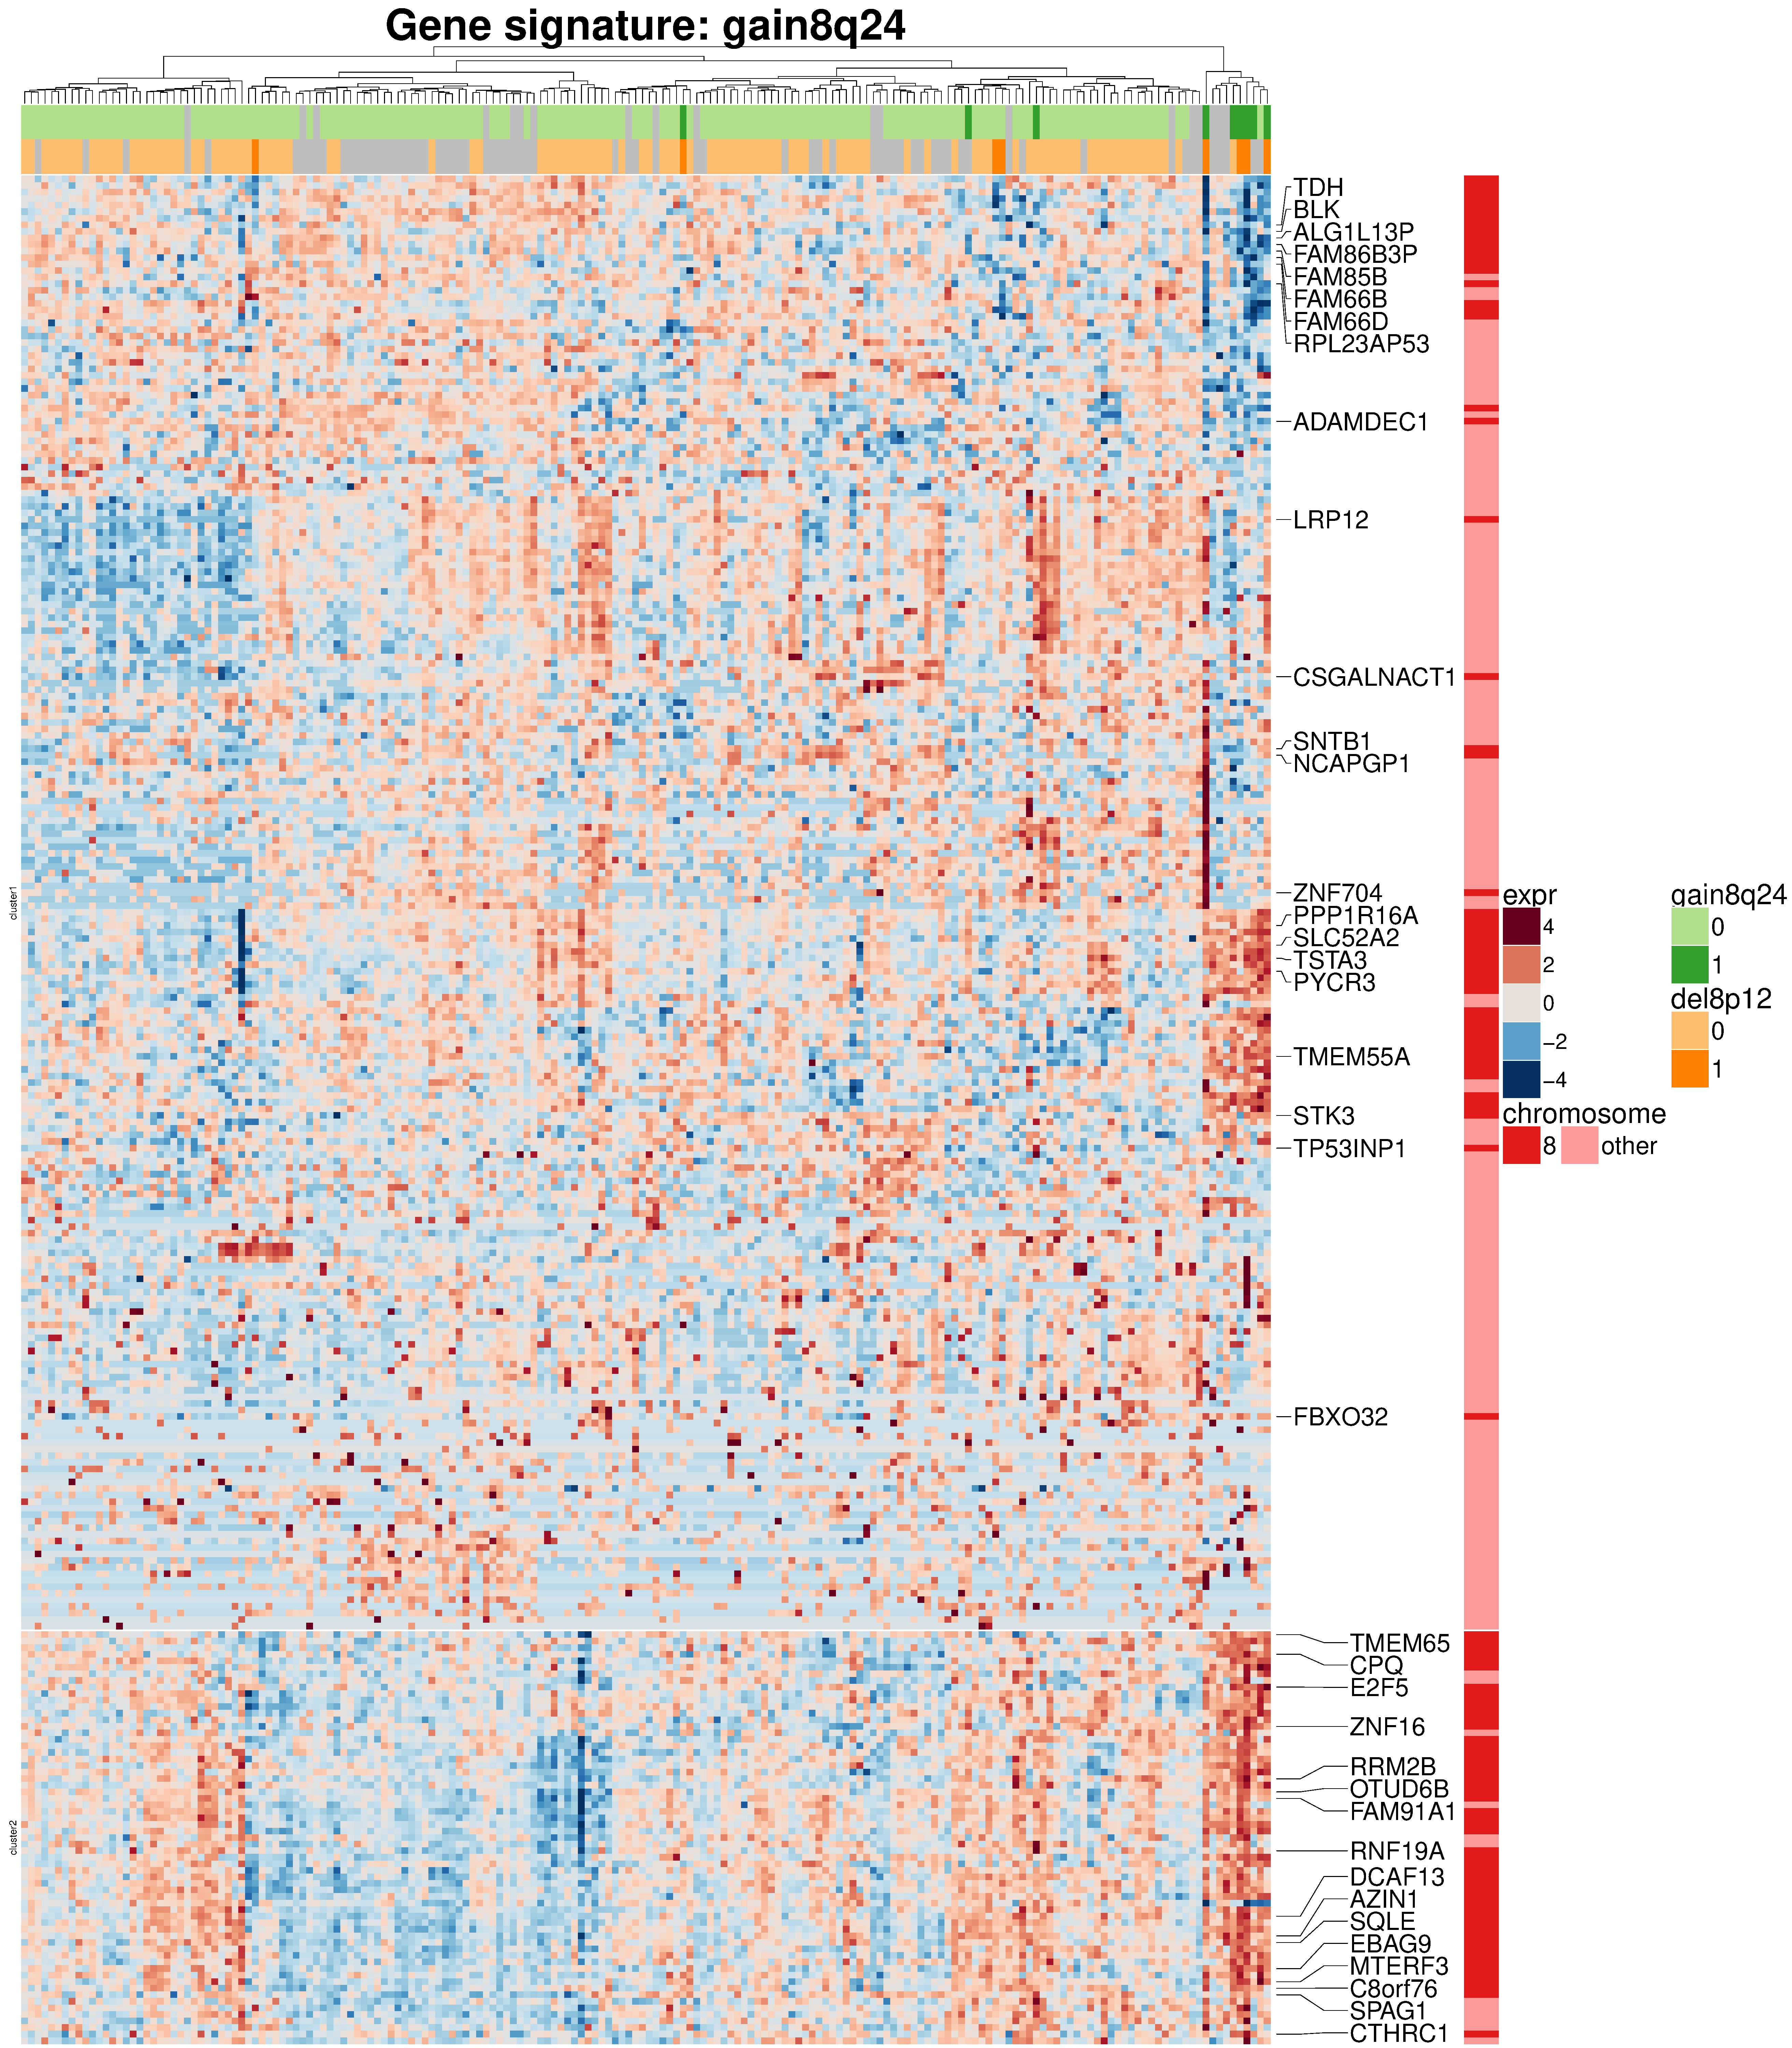
\includegraphics[width=\columnwidth]{./Figures/gene_exprgain8q24_gsea_Hallmark.pdf}
	\caption{\textbf{Gene expression in Gain8q24 and Del8p12:} Differentially expressed genes in Gain8q24 sample cluster by Gain8q24 and Del8p12 revealing interaction of these variants. Thus, we find up and down regulated genes on chromosome 8  among differentially expressed genes. Genes with $\log_2$ fold changes $>2$ on chromosome 8 are annnotated.}
	\label{fig:gene_exprgain8q24_gsea_Hallmark}
\end{figure}

\FloatBarrier


\subsubsection{SF3B1}
Samples with SF3B1 mutation formed a distinct cluster based on differentially expressed genes. 311 genes were significantly up regulated and 162 down regulated ($\text{p}_\text{adj} < 0.01$) (Figure \ref{fig:gene_exprSF3B1_gsea_kegg}). These genes were enriched in metabolic pathways as cholesterol homeostasis, as well as interferon alpha signaling, Notch signaling and Myc targets (see Supplements Figure \ref{fig:Enrichment_others}D). Genes like UQCC1 and EBF1 were significantly up regulated in SF3B1 mutated samples.

\FloatBarrier

\begin{figure}
	\centering
	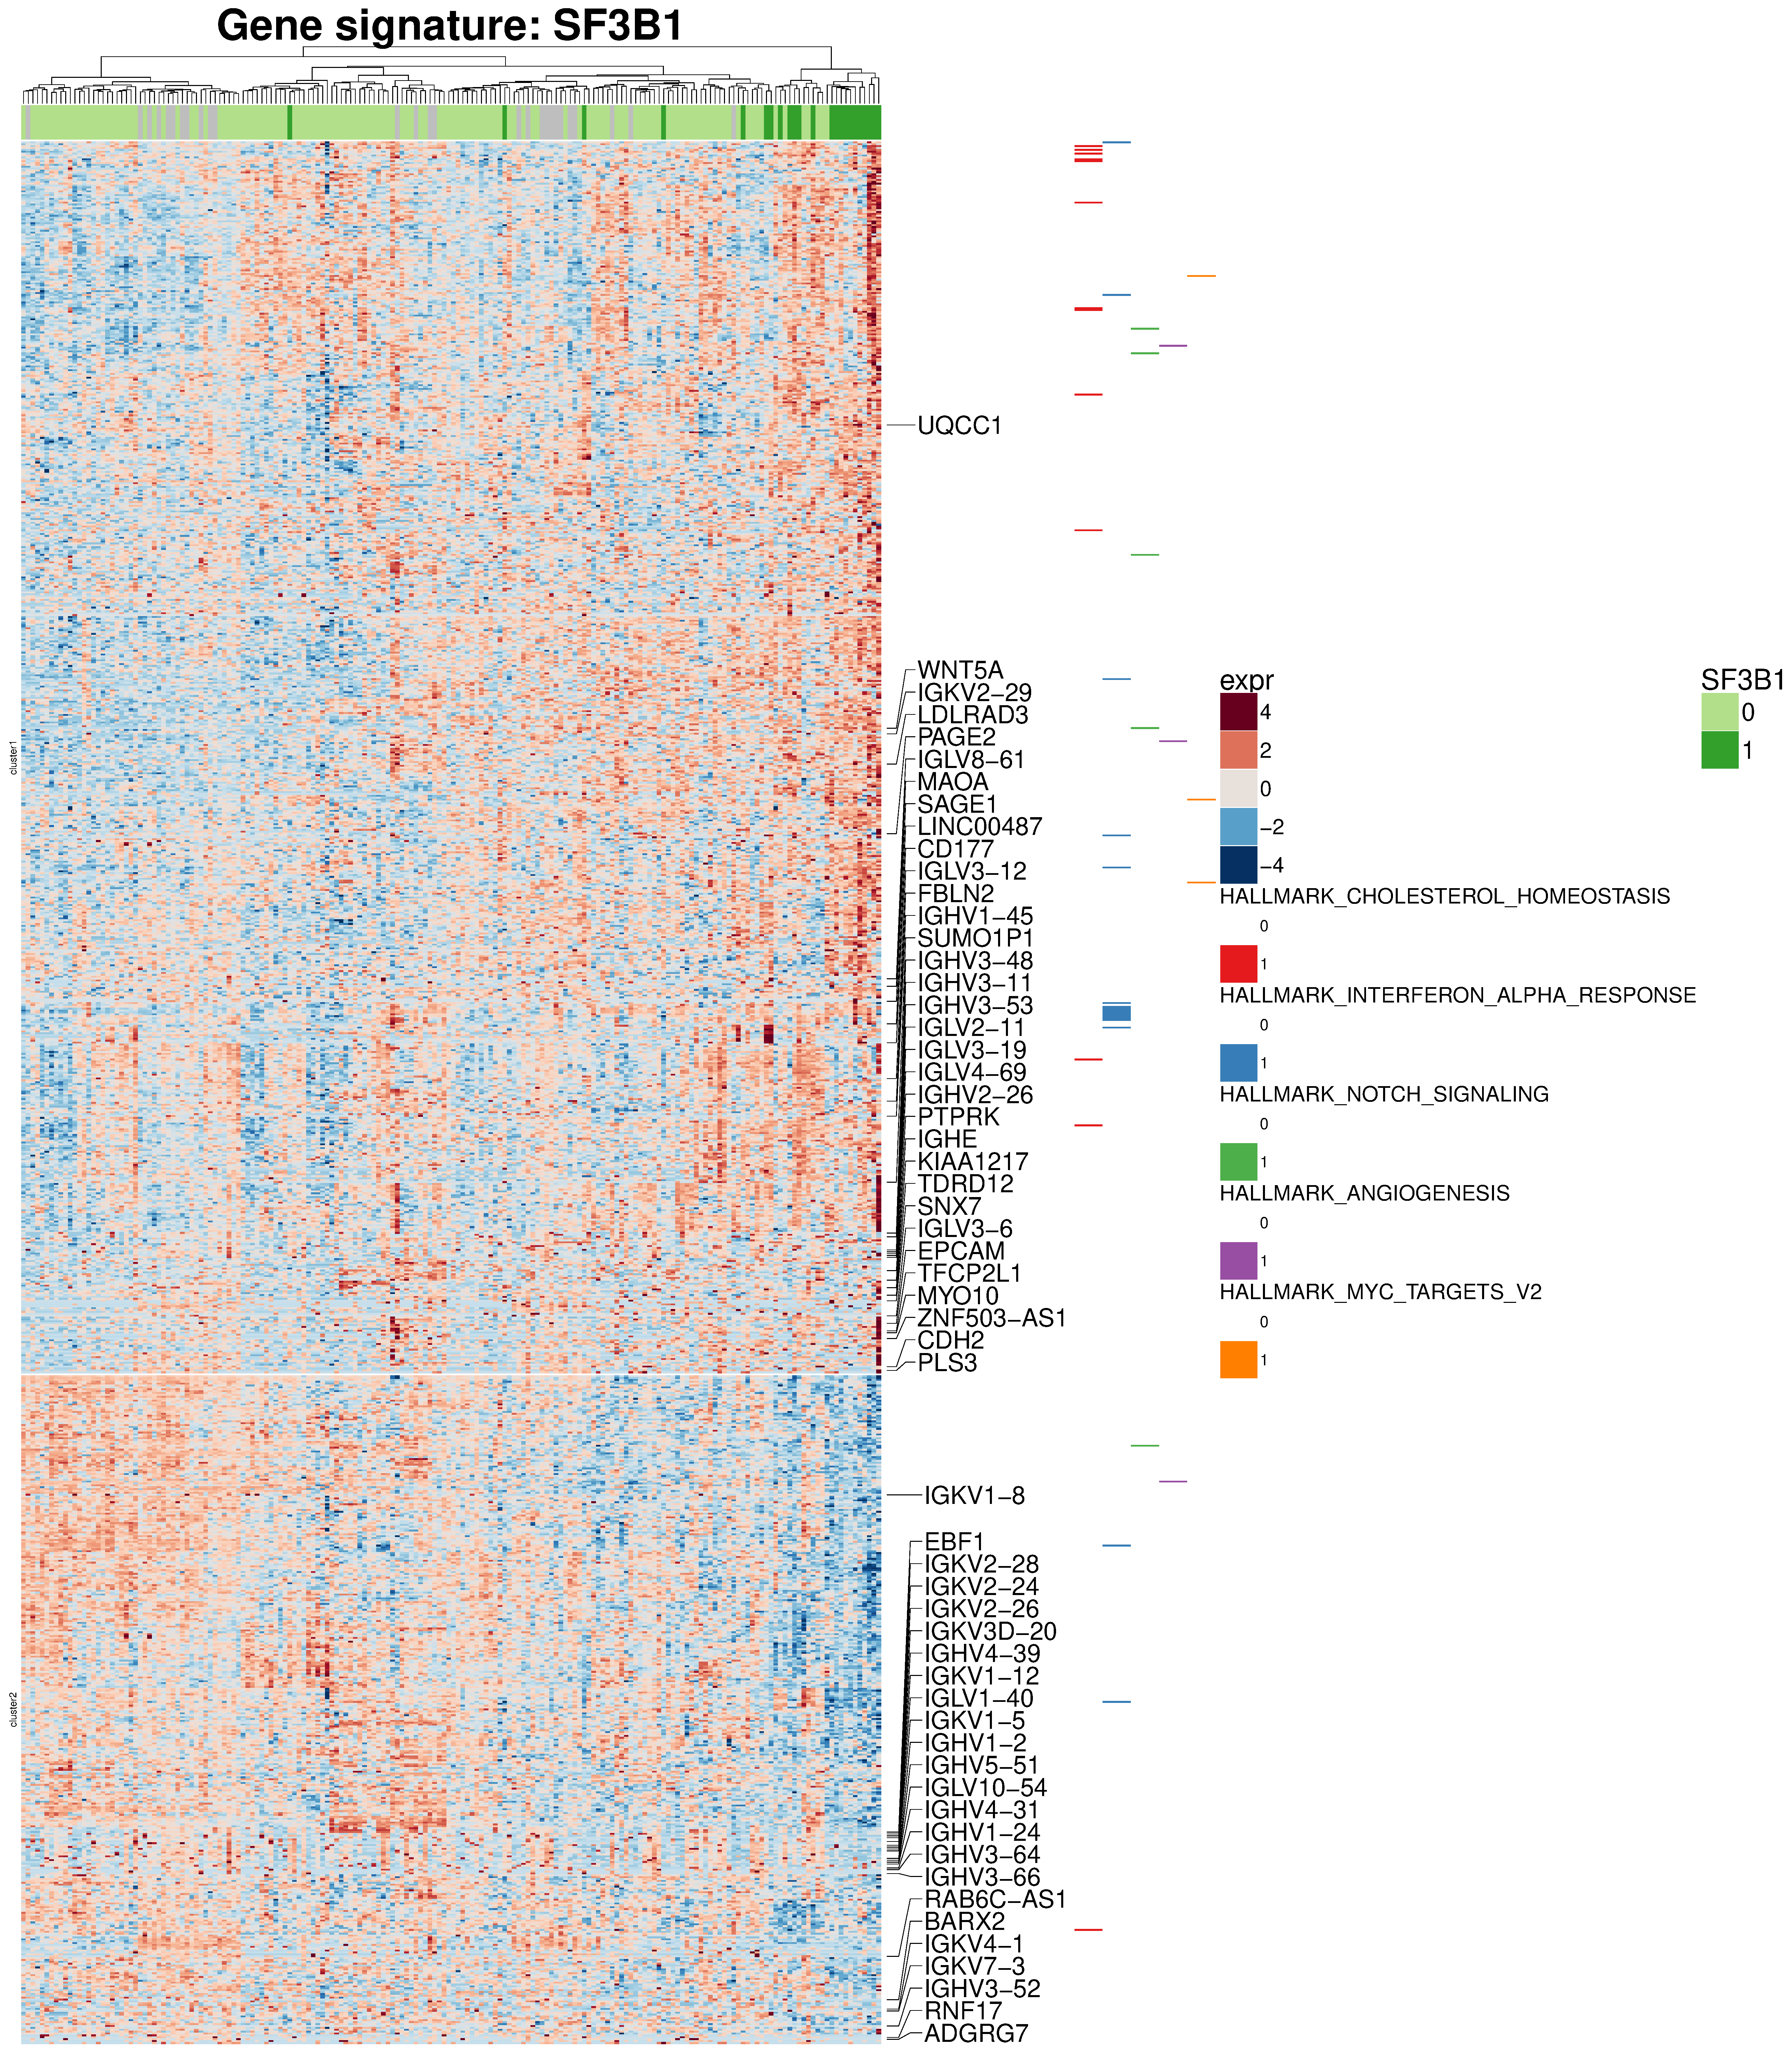
\includegraphics[width=\columnwidth]{./Figures/gene_exprSF3B1_gsea_Hallmark.pdf}
	\caption{\textbf{Gene expression in SF3B1 mutated samples:} Differentially expressed genes in SF3B1 samples form a distinct cluster. SF3B1 mutation is associated with truncated splicing. This leads to coordinated changes on expression level. Genes with $\log_2$ fold change $>4$ are annotated. }
	\label{fig:gene_exprSF3B1_gsea_kegg}
\end{figure}

\FloatBarrier

\subsubsection{BRAF}
Only 3.5\% of PACE samples show a BRAF mutation. Still 678 genes were differentially expressed in this subgroup ($\text{p}_\text{adj} < 0.01$) and BRAF samples formed a distinct cluster. Clear expression pattern were seen in up regulated genes, which were enriched for G2M checkpoint (figure \ref{fig:gene_exprBRAF_gsea_Hallmark}). Down regulated genes did not show consistent pattern among BRAF samples.  

\FloatBarrier

\begin{figure}
	\centering
	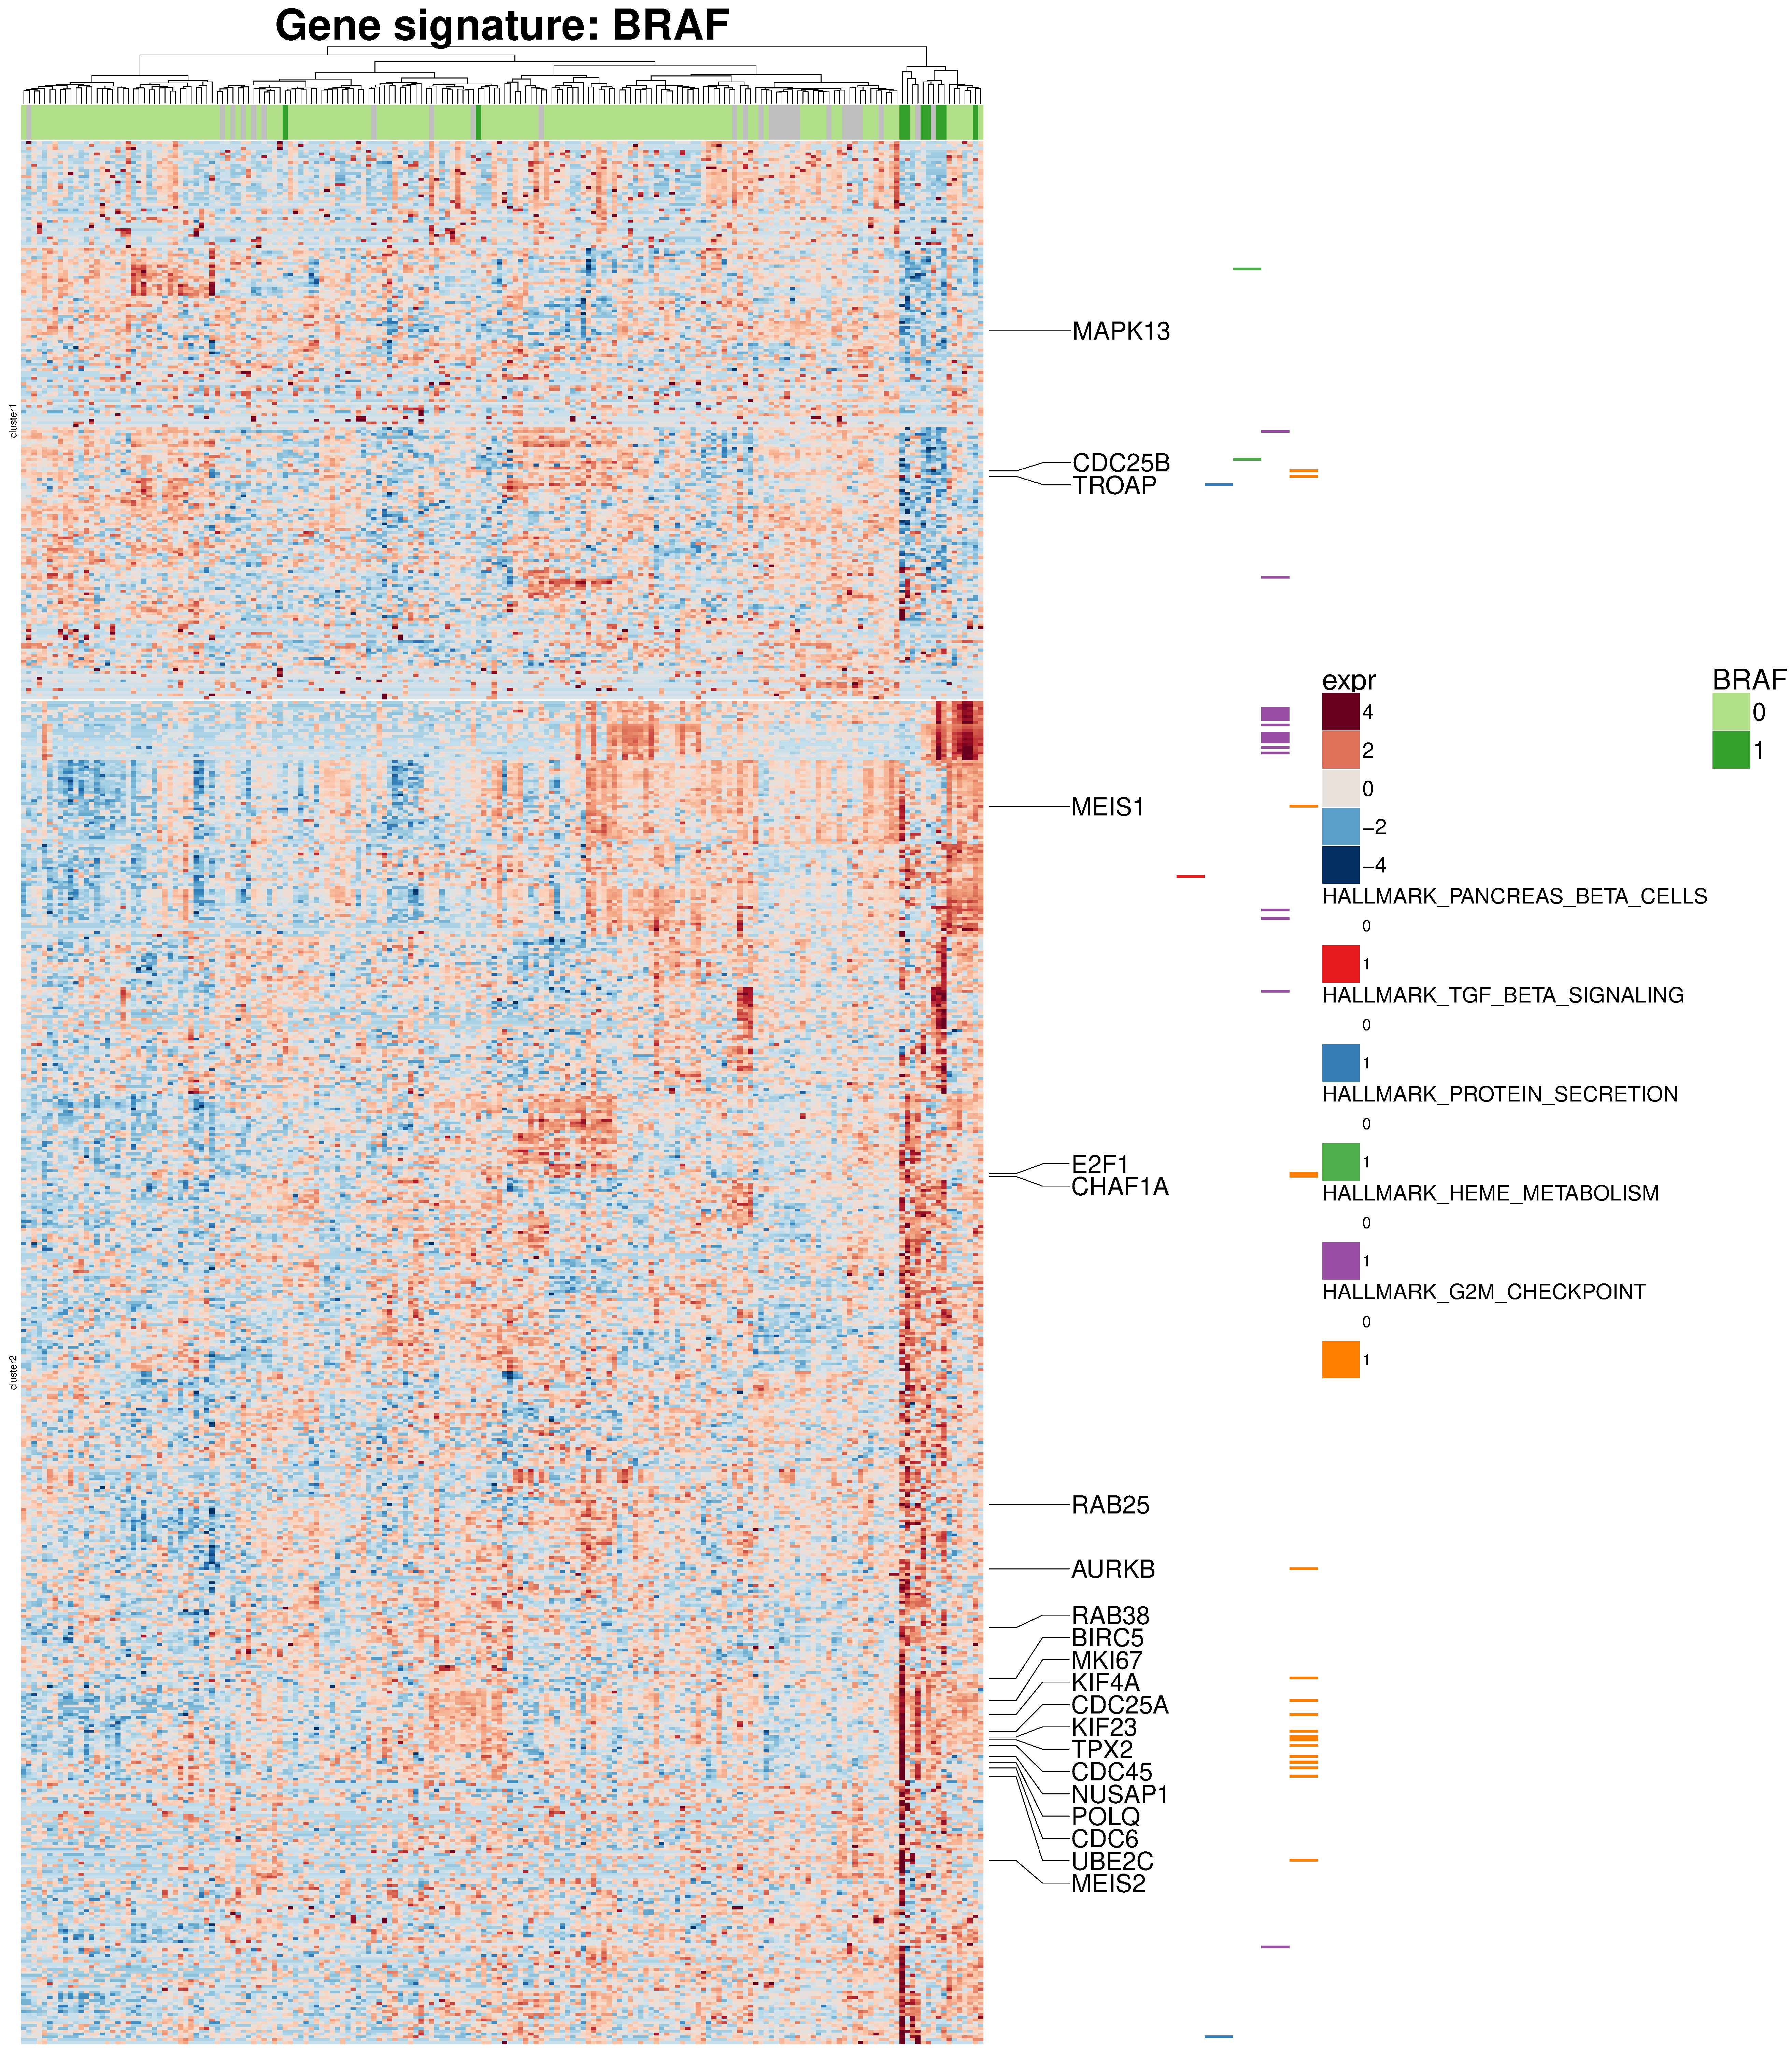
\includegraphics[width=\columnwidth]{./Figures/gene_exprBRAF_gsea_Hallmark.pdf}
	\caption{\textbf{Gene expression in samples with mutated BRAF:} Gene expression in BRAF samples does not show overall coherent cluster. Still a set of up regulated genes that mainly consist of G2M checkpoint genes correlates clearly with BRAF status.}
	\label{fig:gene_exprBRAF_gsea_Hallmark}
\end{figure}

\FloatBarrier
\clearpage

\subsubsection{MED12}
Only 7 of 184 samples show mutated MED12 the PACE dataset did only reveal a few distinct differentially expressed genes (see Supplements Figure \ref{fig:gene_exprMED12_gsea_Hallmark}). MED13L was among down regulated genes. It is part of the mediator complex and supports prior findings \citep{Kampjarvi2015}.

\FloatBarrier


\subsubsection{Notch1}
In total Notch1 mutation was found in 16 samples. 162 genes were differentially expressed ($\text{p}_\text{adj} < 0.05$) between them and other samples in PACE. Despite its adverse clinical prognosis we could not identify distinct gene expression pattern or chromosomal distributions within those (see Supplements Figure \ref{fig:gene_exprNOTCH1_gsea_Hallmark}).

\subsection{Multivariate model}
To account for the effect of co-occurring variants on gene expression we used likelihood ratio tests in differential expression analysis. By comparison of a multivariate model including all variants with a reduced model without the variant of interest we tested for differentially expressed genes in each individual variant controlling for all other variants. As we tested for genes that were solely associated to the individual variants, the numbers of differentially expressed genes were clearly reduced. We still found 1012 genes significantly related to Trisomy12 and 414 related to IGHV status, but for all other variants we found less than 90 and for 5 variants even less than 10 differentially expressed genes (Figure\ref{fig:compModel}). Especially for those variants that were functional correlated, including Del17p13 and TP53 and Del11q22 and ATM, only a few genes were exclusively associated to one variant. The top 7 genes that were differentially expressed in the individual variants are shown in Figure \ref{fig:reducedModel}. We found ATM associated to Del11q22, even when controlling for ATM mutations. Still integrins like ITGF2 were significant in Trisomy12 samples and Notch4 was differentially expressed in Notch1 mutated samples. For Del8p12 the only significant result was KIF13B. This gene is located in the deleted region of Del8p12. These findings are in line with previous results and our expectations. Interestingly, RRM2 was among genes differentially expressed in samples with mutated BRAF.     

\FloatBarrier

\begin{figure}
	\centering
	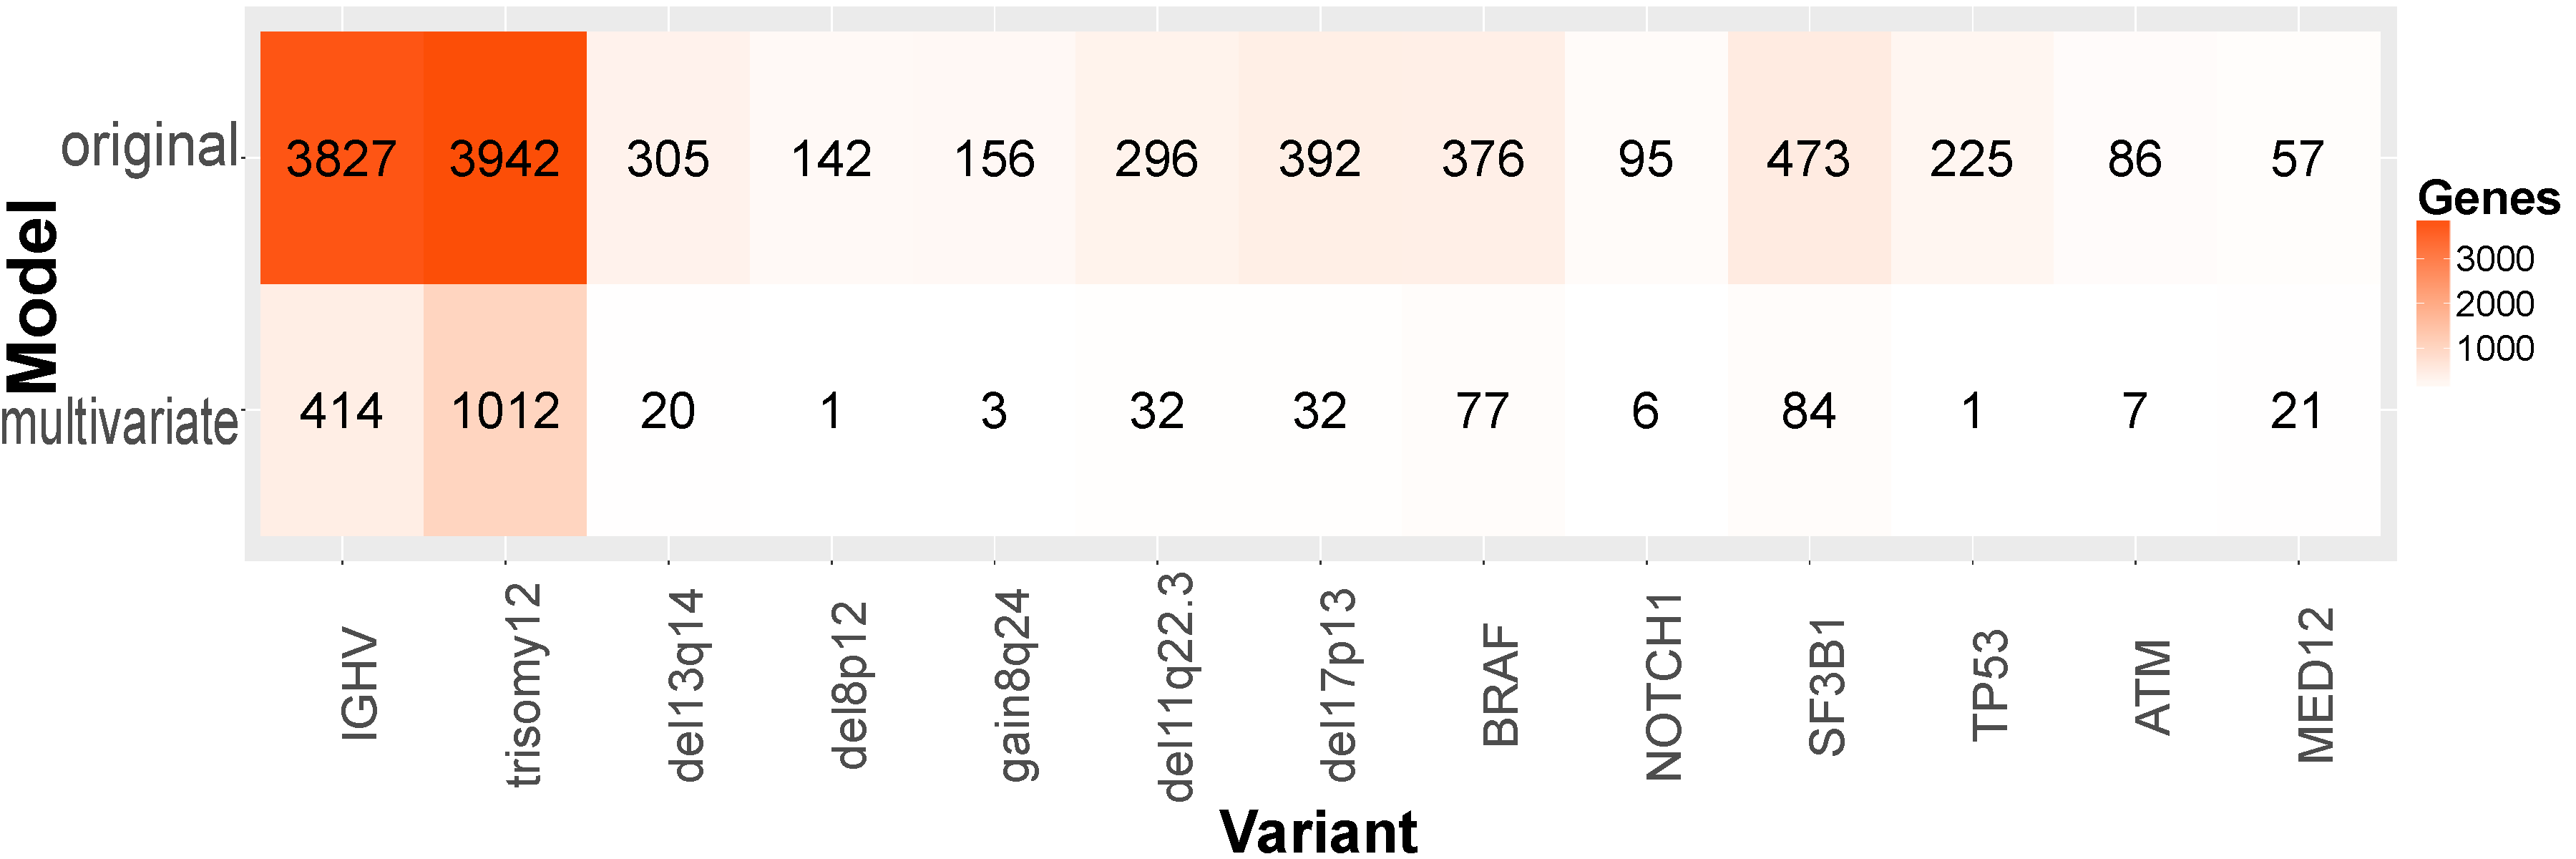
\includegraphics[width=\columnwidth]{./Figures/comparisonModel.pdf}
	\caption{\textbf{Top 7 genes of significant results in the original model and the multivariate model:} For all variants the numbers of differentially expressed genes were clearly reduced when testing for individual variants in a multivariate model against a reduced model by the likelihood ratio test. The original model included IGHV status, Trisomy12 and degree of T cell contamination as covariate. Still 1012 genes are significantly related to Trisomy12 and 414 related to IGHV status, when we control for the effect of confounding variants. Only a few genes are associated to the other variants.}
	\label{fig:compModel}
\end{figure}




\begin{figure}
	\centering
	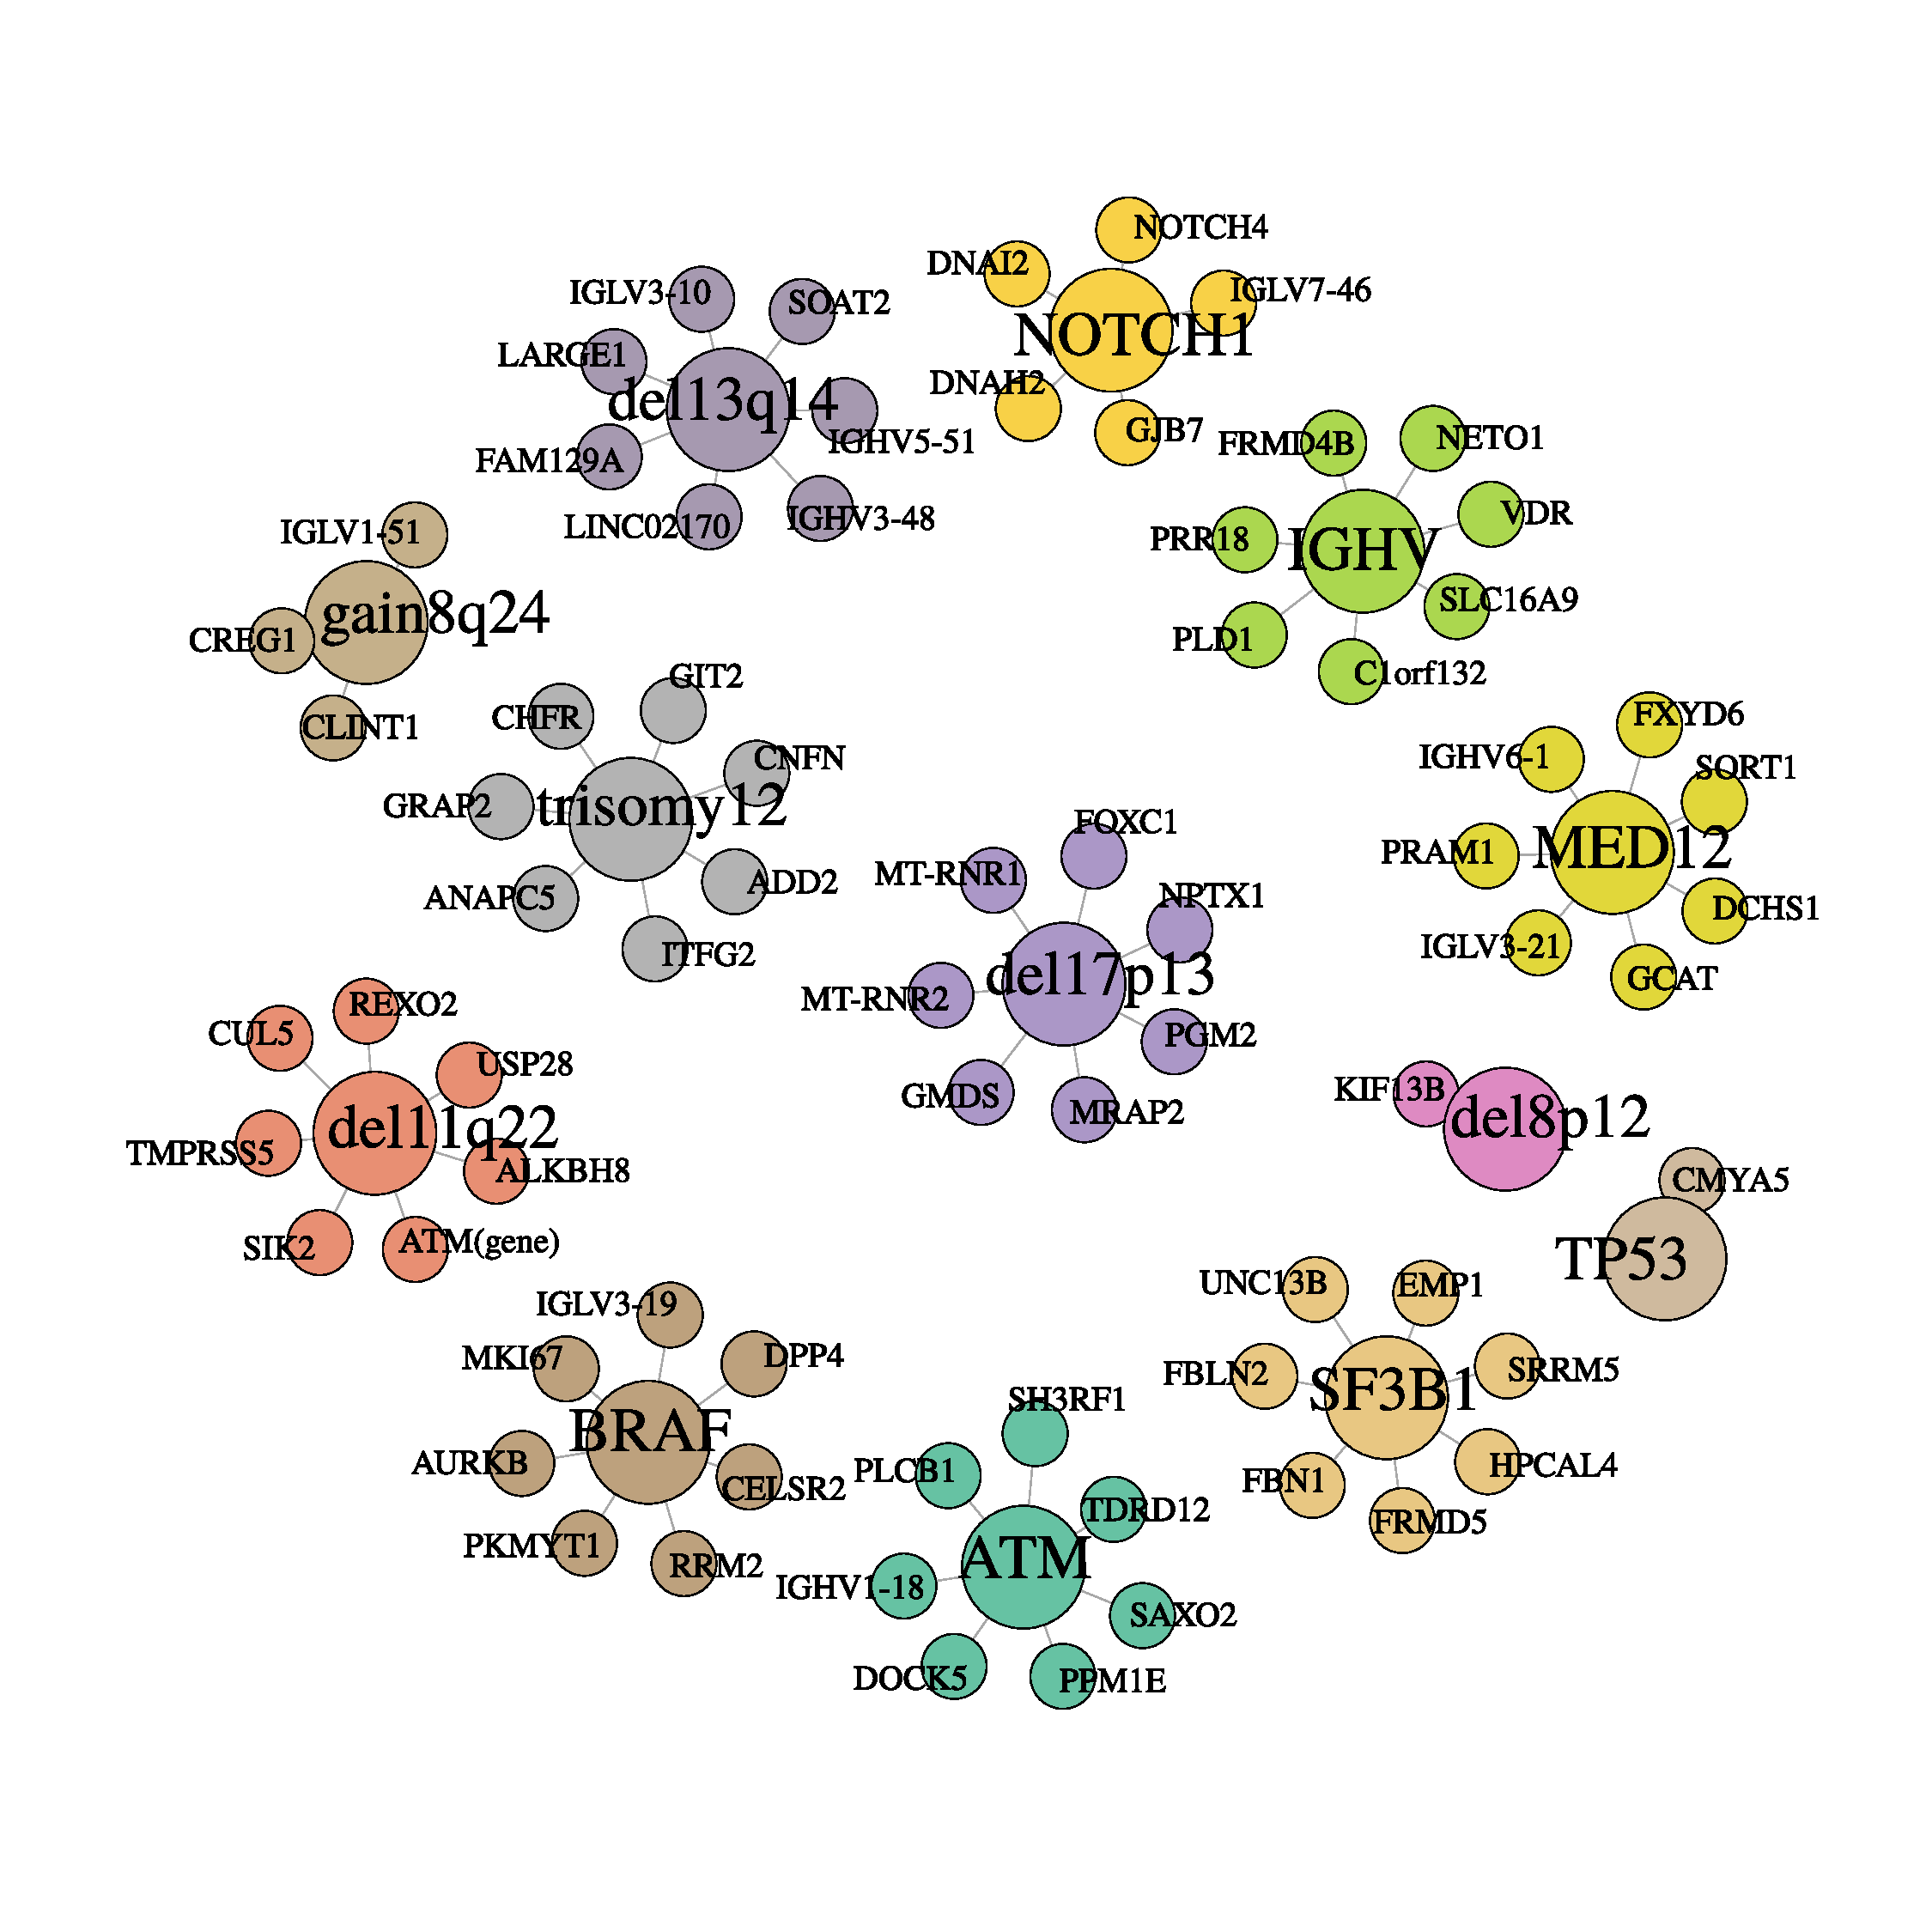
\includegraphics[width=\columnwidth]{./Figures/reducedModel.pdf}
	\caption{\textbf{Most significant differentially expressed genes testing for the effect of each variants alone:} Using a likelihood ratio test to compare a multivariate model with all variants against a reduced model with confounders resulted in small sets of genes related to the individual variants controlling for all other variants. Some of these sets contain less than 7 significant genes. Still we can find known associations like differentially expression of ATM gene in DEL11q22 samples and Notch4 in Notch1 samples.}
	\label{fig:reducedModel}
\end{figure}

\FloatBarrier



\subsection{Methylation profiles in gene expression}
Using the most variant genes, samples formed distinct cluster associated with methylation groups in a PCA (Figure  \ref{fig:pca_Meth_top150}). This indicated an important role of epigenomic regulation in gene expression of CLL. Transcription factor deregulation by differential de-methylation has been suggested as a tumor determining process. EGR1, NFAT and EBF1 were associated with differences in methylation pattern. In line with this, genes of these transcription factors themselves were among genes with highest loadings on PC1, which separated samples by methylation groups. In total 3 out of 4 transcription factors, that have been identified as potentially pathogenic in CLL \citep{Oakes2016}, showed gene expression correlating with methylation groups (Figure \ref{fig:gene_expr_Methylationgroups_top150}). 

\FloatBarrier

\begin{figure}
	\centering
	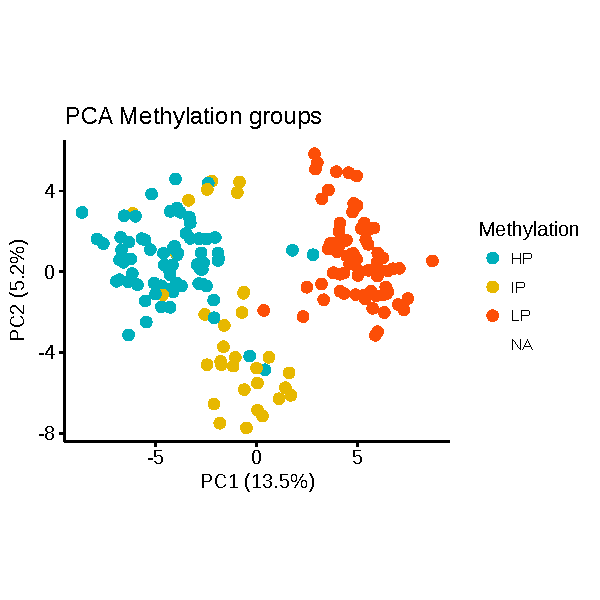
\includegraphics[width=0.75\columnwidth]{./Figures/pca_Meth_top150.pdf}
	\caption{\textbf{Principal component analysis methylation groups:} PC1 and PC2 clearly separate methylation groups into 3 cluster based on expression of the 200 most variable genes.}
	\label{fig:pca_Meth_top150}
\end{figure}


\begin{figure}
	\centering
	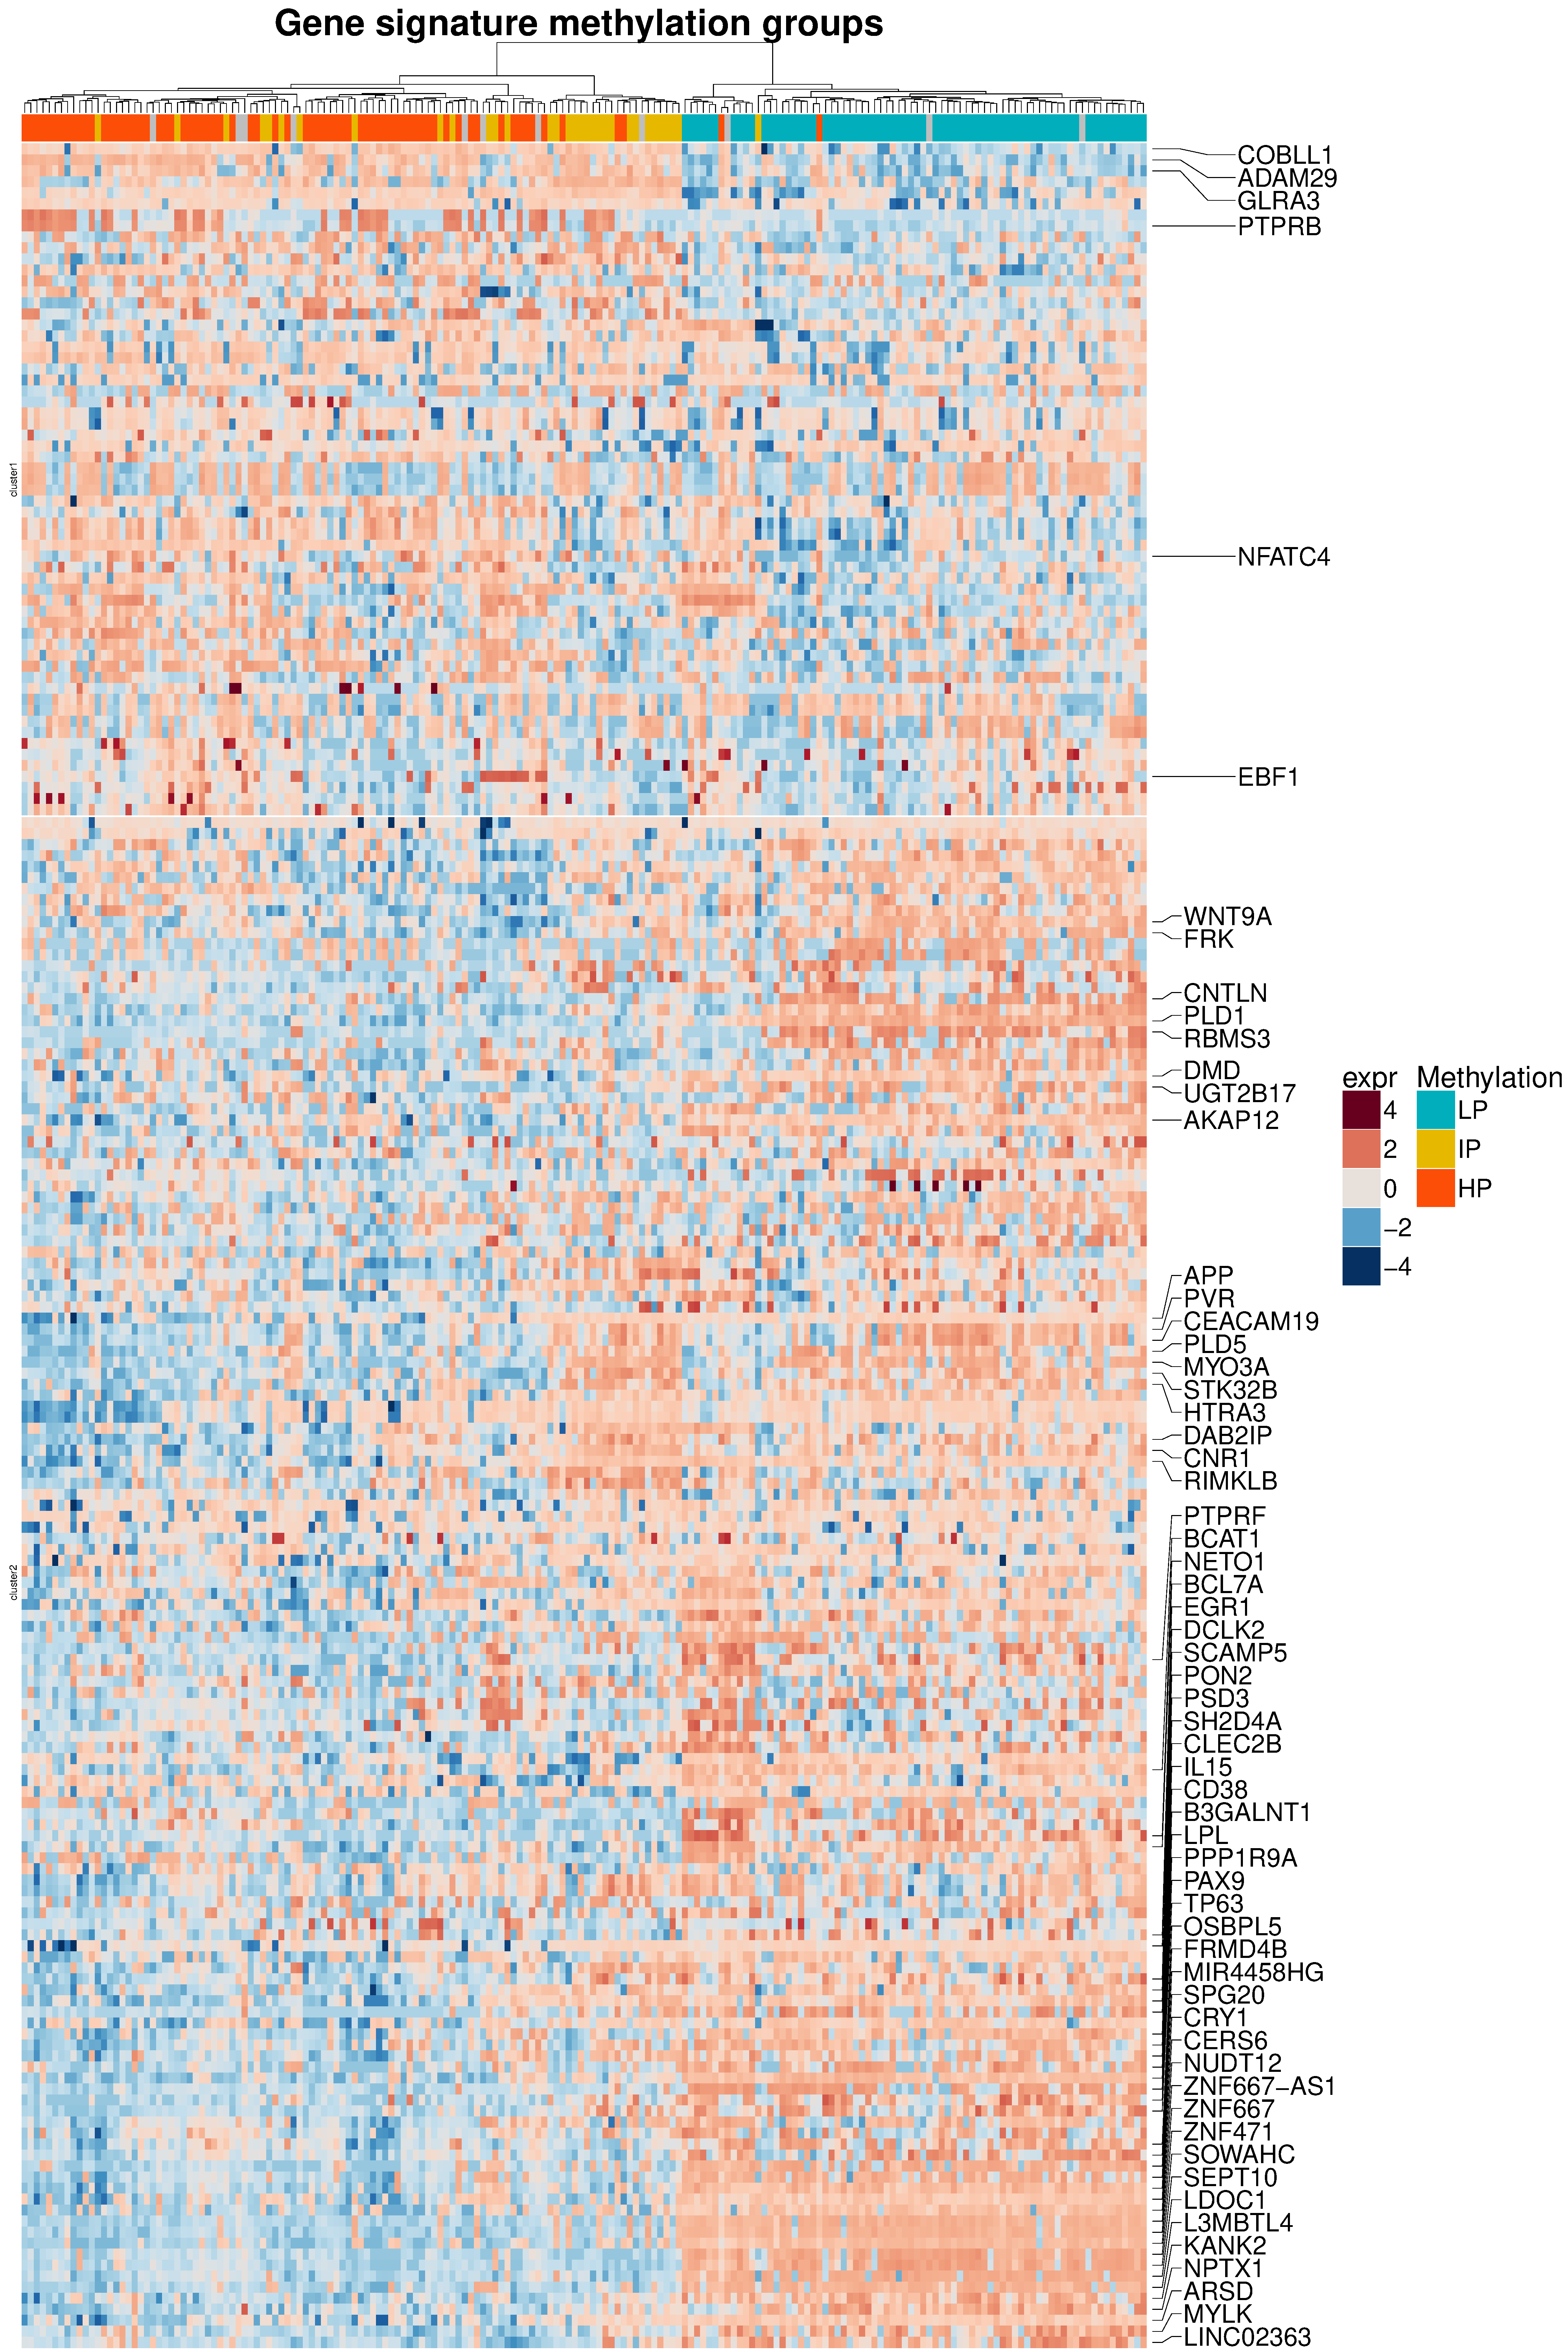
\includegraphics[width=\columnwidth]{./Figures/gene_expr_Methylationgroups_top150.pdf}
	\caption{\textbf{Gene expression of the 200 most variable genes:} The 200 most variable genes show distinct expression within each methylation group. Among them are multifunctional transcription factors like EGR1, NFAT and EBF1.}
	\label{fig:gene_expr_Methylationgroups_top150}
\end{figure}

\FloatBarrier

\subsection{Tumor epistasis in IGHV and Trisomy12}

Differential expression analysis revealed distinct gene signatures between IGHV subtypes and Trisomy12 (Figure \ref{fig:gene_exprIGHV_gsea_hallmark}). Trisomy12 samples formed a separate cluster close to the IGHV mutated samples. Inside this cluster, samples grouped again by IGHV status. It is known that the interplay of different genetic variants characterizes tumorigenesis and can determine cancer phenotype and clinical outcome \citep{Landau2015}. We show here, that gene expression data can also reflect this interplay between Trisomy12 and IGHV hypermutations. The combined genotype showed different expression pattern from what would have been expected from the individual effects of the variants. Modeling gene expression as epistatic interaction resulted in 602 significantly associated genes in the presence of IGHV hypermutations and Trisomy12, together or alone (Figure \ref{fig:epistasisTri12IGHV}). They formed 5 cluster with distinct gene expression patterns, suggesting different layer of interactivity. The first cluster represented genes only down regulated in IGHV unmutated samples. A subset of these genes was located on chromosome 12, which could be a reason why down regulation failed in Trisomy12 samples with unmutated IGHV status. Further clusters showed strong up resp. down regulation in CLL-M samples with Trisomy12. These clusters showed clear interaction on gene expression level between Trisomy12 and IGHV. Significantly up-regulated genes were CD38, MAP3K8 and CDCP1. Another gene cluster represented genes up regulated in Trisomy12 samples without IGHV mutations. In the presence of both trisomy12 and IGHV mutation, the up regulation of those genes were suppressed. As described by Fischer et al. [2015], we inferred directions for each gene describing the interactions as one variant alleviating or aggravating the effect of the other. Interestingly, we observed consistent directions within gene clusters. This confirmed our observation, that the clusters represent different layer of interactivity. In the cluster with enhanced expression in M-CLL with Trisomy12 the interaction was directed from IGHV to Trisomy12, whereas in the cluster with genes down regulated in IGHV unmutated samples, the presence of Trisomy12 determined the effect of the IGHV status on gene expression.       


\FloatBarrier

\begin{figure}
	\centering
	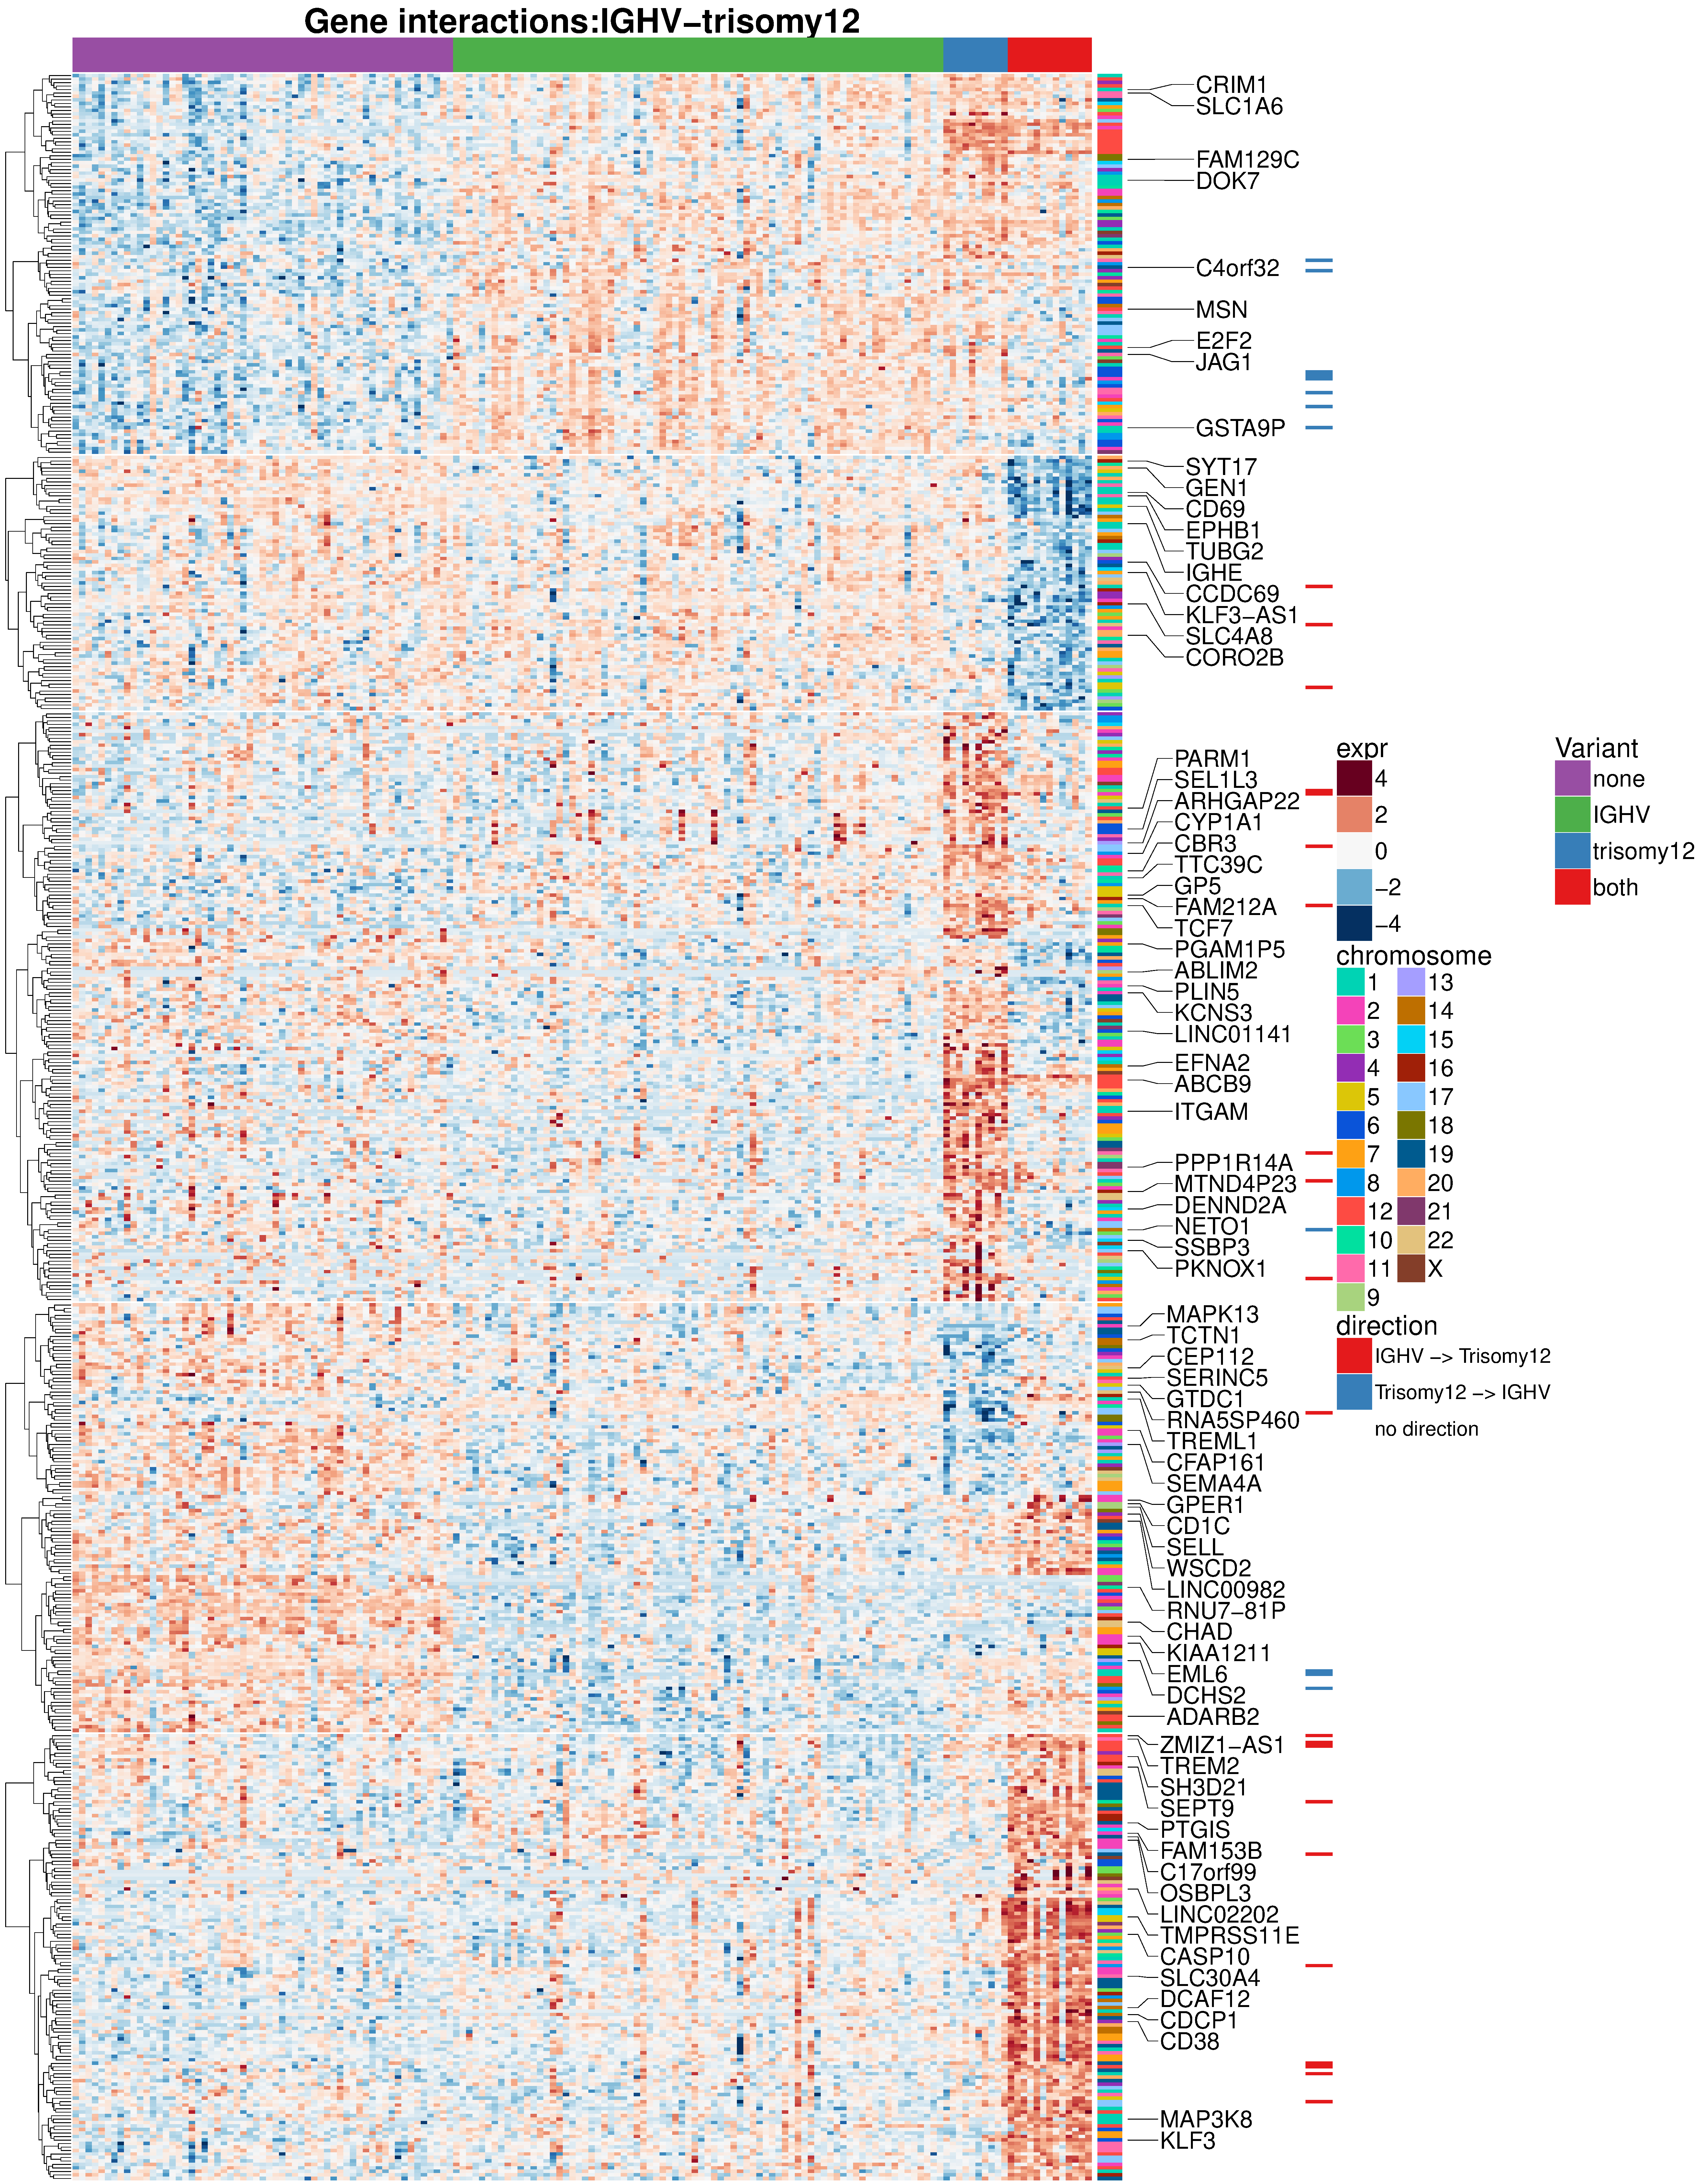
\includegraphics[width=\columnwidth]{./Figures/epistatsisTri12IGHV.pdf}
	\caption{\textbf{Genes differentially expressed between samples with Trisomy12, IGHV mutated, both or IGHV-unmutated genotypes:} Genes can be distinguished into 5 groups revealing clear patterns of interactivity. The direction of interaction is consistent within these clusters.}
	\label{fig:epistasisTri12IGHV}
\end{figure}

\FloatBarrier

